\documentclass[12pt]{report}

\usepackage[french]{babel}
\usepackage[utf8]{inputenc}%pour le é 
\usepackage[T1]{fontenc}
\usepackage{fancyhdr}%pour l'en-tete 
\usepackage{graphicx}%pour les images
\usepackage[margin=1in]{geometry}
\usepackage{cite}%pour bibliographie 
\usepackage{wrapfig} %pour figure a coté du texte
\frenchbsetup{StandardLists=true} % à inclure si on utilise \usepackage[french]{babel}
\usepackage{enumitem}
\usepackage{amssymb}
\usepackage[section]{placeins}

%		Header		%		
\usepackage{fancyhdr}
\pagestyle{fancy}
\rhead{\thepage}
\lhead{\leftmark}

\usepackage{makeidx}
\makeindex
\usepackage[sort=use]{glossaries}

\makeglossaries
 

\newcommand\tab[1][0,4cm]{\hspace*{#1}}
\newcommand\longtab[1][1cm]{\hspace*{#1}}



\begin{document}

\thispagestyle{empty}

\addcontentsline{toc}{chapter}{Remerciements}

\vspace*{5cm}

\begin{center}
\textbf{Remerciements}
\end{center}

\input{Parts/resume.tex}


\listoffigures  % table des figures
\listoftables

\printglossaries
\tableofcontents

 % \newcommand\tab[1][0,4cm]{\hspace*{#1}}
\newcommand\longtab[1][1cm]{\hspace*{#1}}
% \setlength{\headheight}{15pt}



\chapter{Generalités sur les applications mobiles}
\section{Introduction}
\tab Dans ces derniers temps, la possession d'un smartphone ou une tablette est devenue indispensable dans notre vie quotidienne, ces derniers sont gérés par de nombreux systèmes d'exploitation.\medskip
\\
Les systèmes d'exploitation sont des logiciels conçus pour faire fonctionner un smartphone en permettant à l'utilisateur de réaliser plusieurs tâches comme passer un appel, prendre des photos et même télécharger des applications pour mieux exploiter son smartphone.\medskip
\\
Dans ce chapitre nous allons nous focaliser sur les différents systèmes d'exploitation et le développement des applications mobiles , nous commençons par une définition d'Android et IOS, ensuite nous allons faire une comparaison entre les deux systèmes d'exploitation et pour finir , nous allons parler sur le développement des applications mobiles et les différents outils utilisés dans ce domaine.\medskip

\section{Les systèmes d'exploitation mobiles}
\subsection{Définition}
Un système d'exploitation mobile est un système d'exploitation conçu pour fonctionner sur un appareil mobile. Ce type de système d'exploitation se concentre entre autres sur la gestion de la connectivité sans fil et celle des différents types d'interface.~\cite{SystemeExploitationMobile}

Les systèmes d'exploitation mobiles sont généralement installés sur les smartphones. Il existe un grand nombre de systèmes d'exploitation tel que : Windows Phone, iOS, Android, BlackberryOs, Symbian OS et Bada.

Les deux systèmes d'exploitation les plus présents en ce temps sont Android de l'entreprise Google et iOS d'Apple. Ces deux systèmes offrent de manière régulière des mises à jour qui améliorent la qualité et les performances du système en plus de renforcement de la sécurité de l'appareil.
 

\subsection{Le système Android}
\begin{wrapfigure}[8]{r}{3cm}
    \vspace{-15pt}
    
\includegraphics[width=3cm]{images/Chapitre1/android.jpg}
    \vspace{-20pt}
    \caption{{\footnotesize Logo Android}}
\end{wrapfigure}



Android est un système d'exploitation créé par Google, ce système permet d'utiliser son smartphone, le personnaliser et même télécharger des applications pour faciliter les tâches quotidiennes de l'utilisateur et mieux exploiter son appareil.

Lancé en juin 2007 à la suite du rachat par Google en 2005 de la startup du même nom6, le système avait d'abord été conçu pour les smartphones et tablettes tactiles, puis s'est diversifié dans les objets connectés et ordinateurs comme les télévisions (Android TV), les voitures (Android Auto), les Chromebook (Chrome OS qui utilise les applications Android) et les smartwatch (Wear OS).~\cite{AndroidWikipedia}

Le système Android a été développé et ce jusqu'à la version 10 appelée Android Q. Ce système est distribué vers les smartphones et les tablettes sous trois formes : 
\begin{itemize}
    \item Un système d'exploitation customisé en appliquant une surcouche logicielle qui va avec les modèles de chaque constructeur comme One UI de Samsung, MIUI de Xiaomi et EMUI de Huawei. cela apporte une meilleure expérience utilisateur
   
    \begin{figure}[!ht]
        \centering
        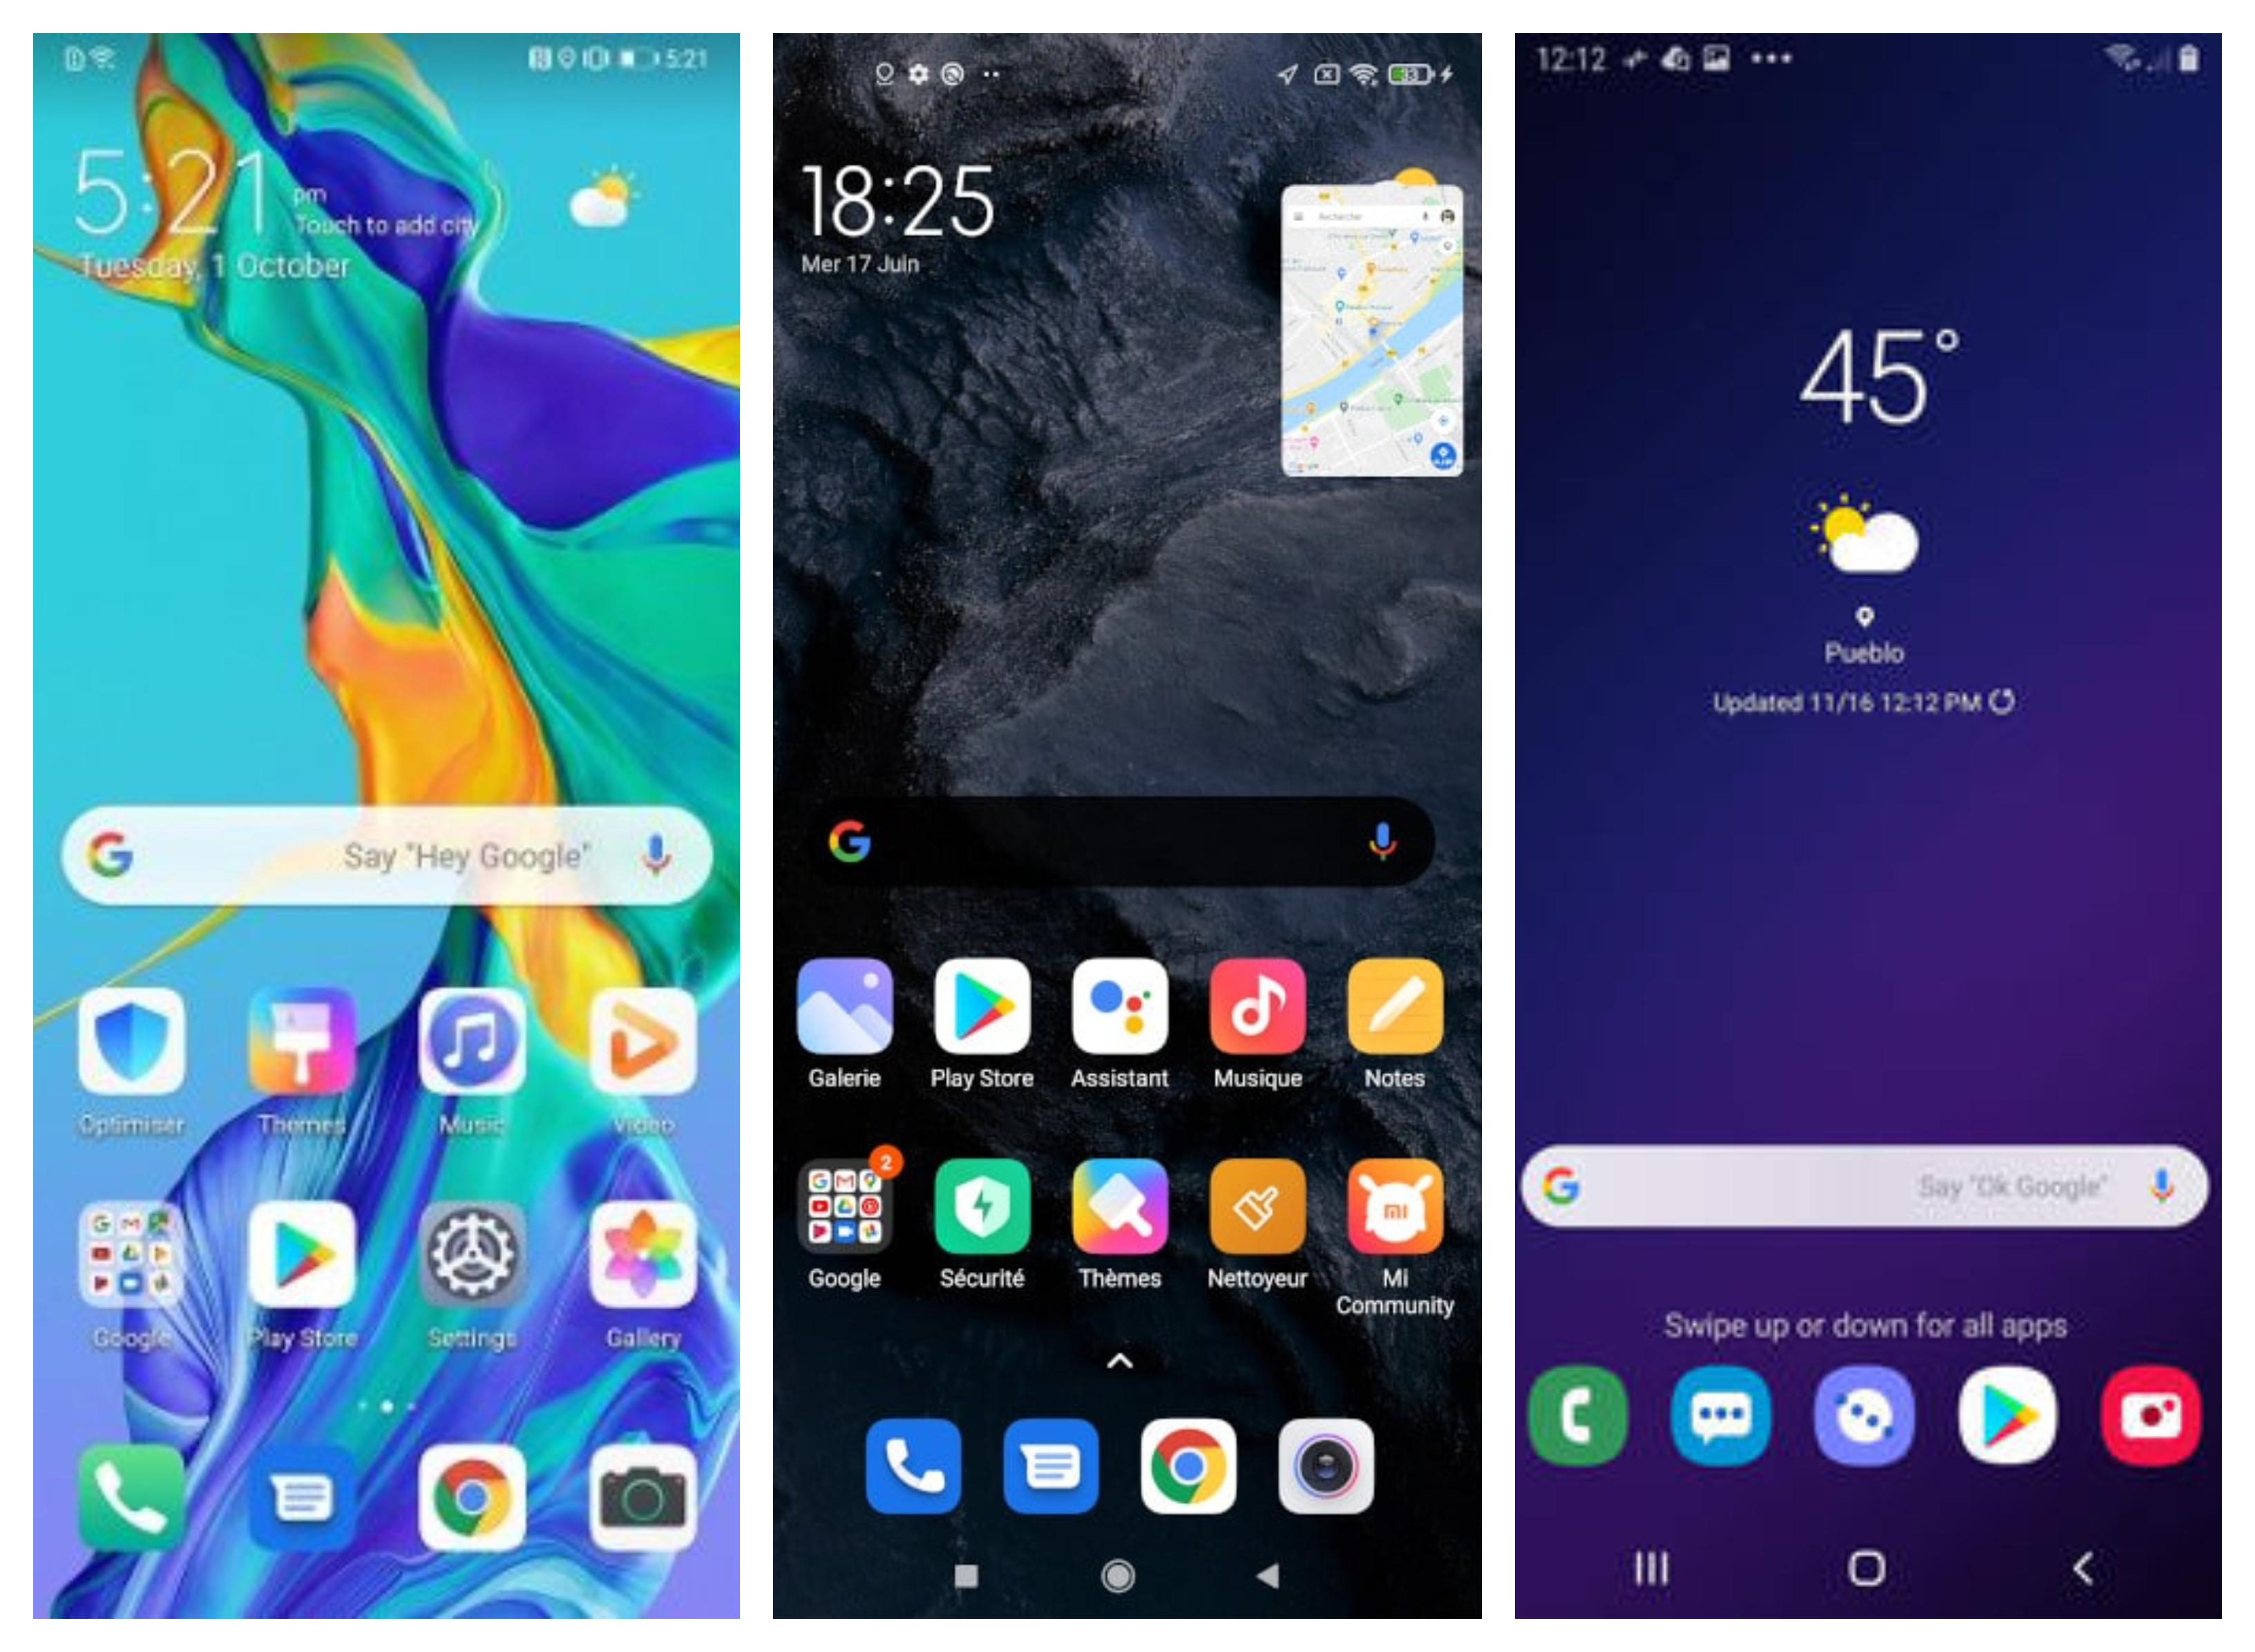
\includegraphics[width=4in]{images/Chapitre1/surcouche.jpg}
        \label{fig:surcouche}
        \caption{Différence entre les surcouches EMUI, MIUI et ONE UI}
    \end{figure}

    \item Un système d'exploitation sans  l'application d'une surcouche. cette version est installé par exemple sur les smartphones Android Go, Ces derniers sont mis à jour rapidement vers de nouvelles versions de ce système.
    \begin{figure}[!ht]
        \centering
        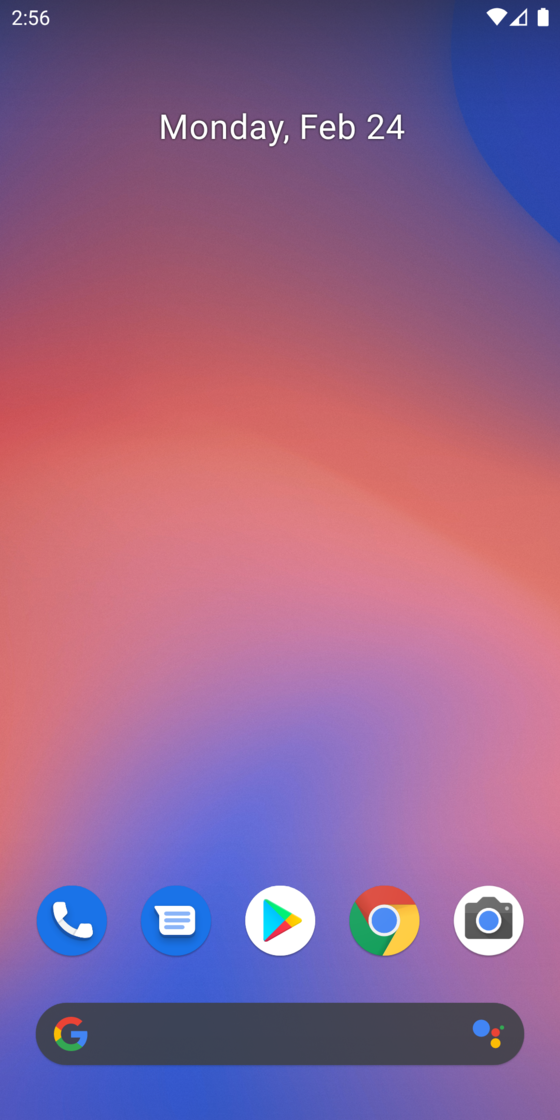
\includegraphics[width=1.5in]{images/Chapitre1/android_R.png}
        \label{fig:androidsanssurcouche}
        \caption{L'interface utilisateur d'Android 10 sans l'application des surcouches}
    \end{figure}
    \item Le système Android est installé aussi sous la forme de versions alternatives appelées Custom ROM. On installe ces ROM par exemple lorsqu'un smartphone est incompatible avec une version Android, ce ROM s'installe avec la version courante d'Android mais avec une interface d'un système différent.
\end{itemize}
\newpage
\tab \textbf{L'architecture d'Android:}\medskip

L'architecture du système Android est sous forme d'une pile de composants comme on le voit dans la figure suivante :
\begin{figure}[!ht]
    \centering
    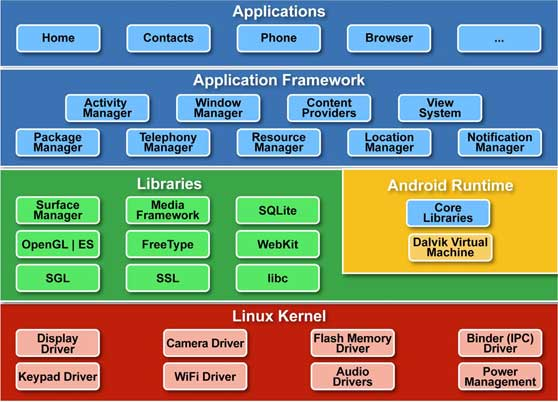
\includegraphics[width=5in]{images/Chapitre1/android_architecture.jpg}
    \label{fig:architecture android}
    \caption{L'architecture d'Android}
\end{figure}

En lisant la figure de bas en haut, on trouve dans la première couche que ce système est basé sur le noyau (ou Kernel) de Linux conçu spécialement pour l'environnement mobile, ce composant joue le rôle d'un pont entre les composants matériels et logiciels. Il contient donc tous les pilotes, ces derniers utilisent des fonctions qui permettent de contrôler le matériel.

Au-dessus du kernel il y a le "Hardware abstraction layer" qui permet de séparer la plateforme logique du matériel. Au-dessus de cette couche d'abstraction on retrouve les librairies C./C++ utilisées par un certain nombre de composants du système Android.
On retrouve ensuite l'Android Runtime, cette couche contient les librairies cœurs du Framework ainsi que la machine virtuelle exécutant les applications. Au-dessus la couche "Android Runtime" et des librairies cœurs on retrouve le Framework permettant au développeur de créer des applications.
Enfin au-dessus du Framework il y a les applications.

\subsection{Le système iOS}
\begin{wrapfigure}[8]{r}{3cm}
    \vspace{-15pt}
    
\includegraphics[width=3cm]{images/Chapitre1/ios_logo.jpg}
    \vspace{-20pt}
    \caption{{\footnotesize Logo iOS}}
\end{wrapfigure}

iOS, anciennement iPhone OS , est le système d'exploitation mobile développé par Apple pour plusieurs de ses appareils. Il est dérivé de macOS dont il partage les fondations (le noyau hybride XNU basé sur le micro-noyau Mach, les services Unix et Cocoa, etc.).

iOS comporte quatre couches d'abstraction, similaires à celles de macOS : une couche « Core OS », une couche « Core Services », une couche « Media » et une couche « Cocoa ». Le système d'exploitation occupe au maximum 3 Go de la capacité mémoire totale de l'appareil, selon l'appareil.~\cite{IOS2020}

Ce système d'exploitation est connu par sa rapidité et fluidité sur les appareils d'Apple vu qu'il est développé spécialement pour les iphones contrairement à Android.

\begin{figure}[!ht]
    \centering
    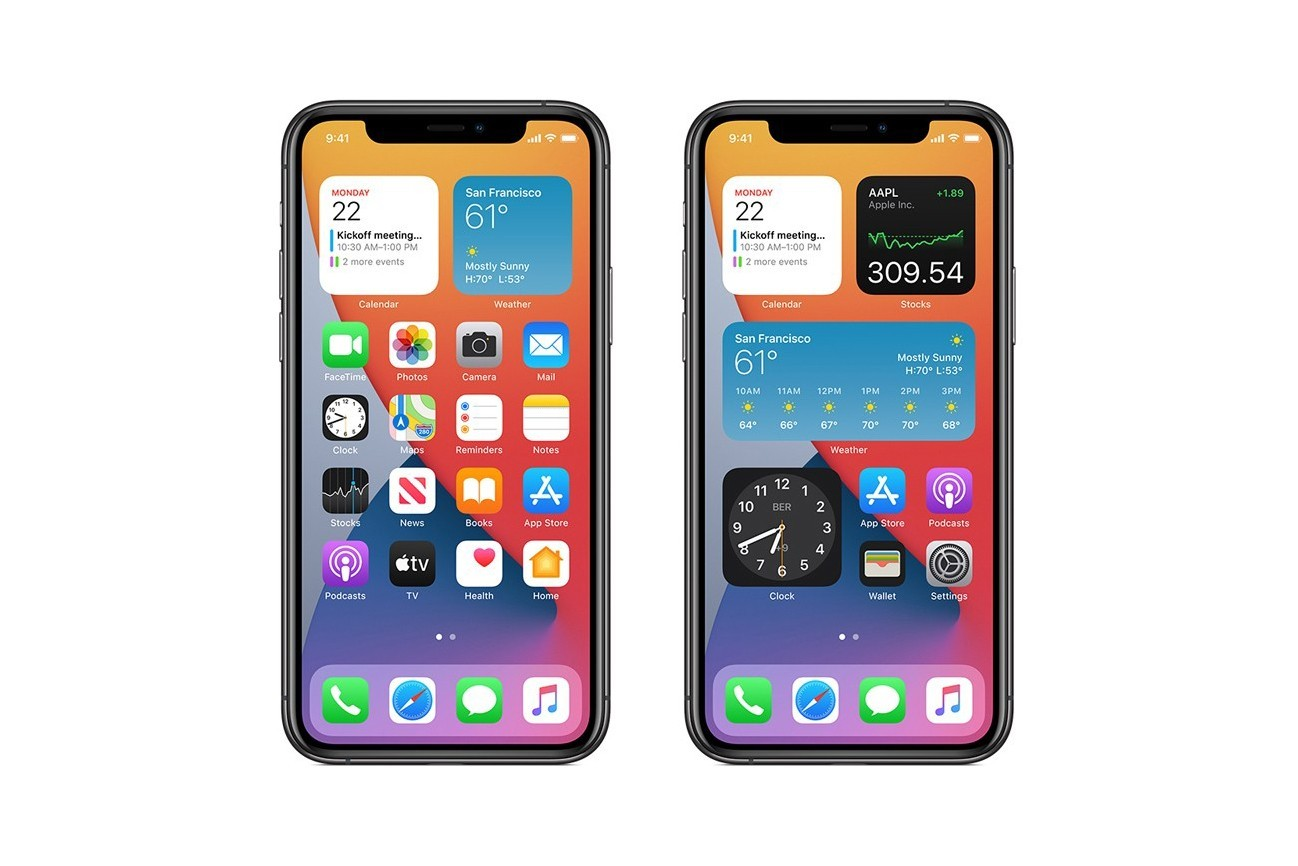
\includegraphics[width=5in]{images/Chapitre1/iosui.jpg}
    \label{fig:ios Ui}
    \caption{L'interface de iOS}
\end{figure}
\newpage
\tab \textbf{L'architecture d'iOS:}\medskip

Comme on l'a déjà mentionné dans la partie précédente, iOS est basé sur macOS. Son architecture est composée de 4 éléments: le BaseBand, le BootLoader,le Firmware et le SeckPack.

\begin{itemize}
    \item Le BaseBand est un micrologiciel autonome qui gère en temps réel tous les périphériques de communication de l'appareil. Le BaseBand est considéré donc comme le BIOS de l'iPhone.
    \item Le BootLoader est le programme chargé du démarrage du système iOS, c'est le premier processus exécuté lorsqu'on allume l'iphone 
    \item Le Firmware est un programme interne dans l'iPhone, ce programme prend contrôle de la partie systématique de l'appareil comme la caméra, l'écran et le clavier tactile. 
    \item Le SeckPack est une partie de la mémoire flash de l'appareil contenant entre autres des informations sur le verrouillage de celui-ci. Le Seckpack peut être considéré comme un mot de passe : en effet, si un SeckPack correct est fourni au BootLoader lors du lancement, alors l'utilisateur a la possibilité d'utiliser le BaseBand, et donc les fonctionnalités de téléphonie et d'Internet.~\cite{IOS2020}
\end{itemize}

\begin{figure}[!ht]
    \centering
    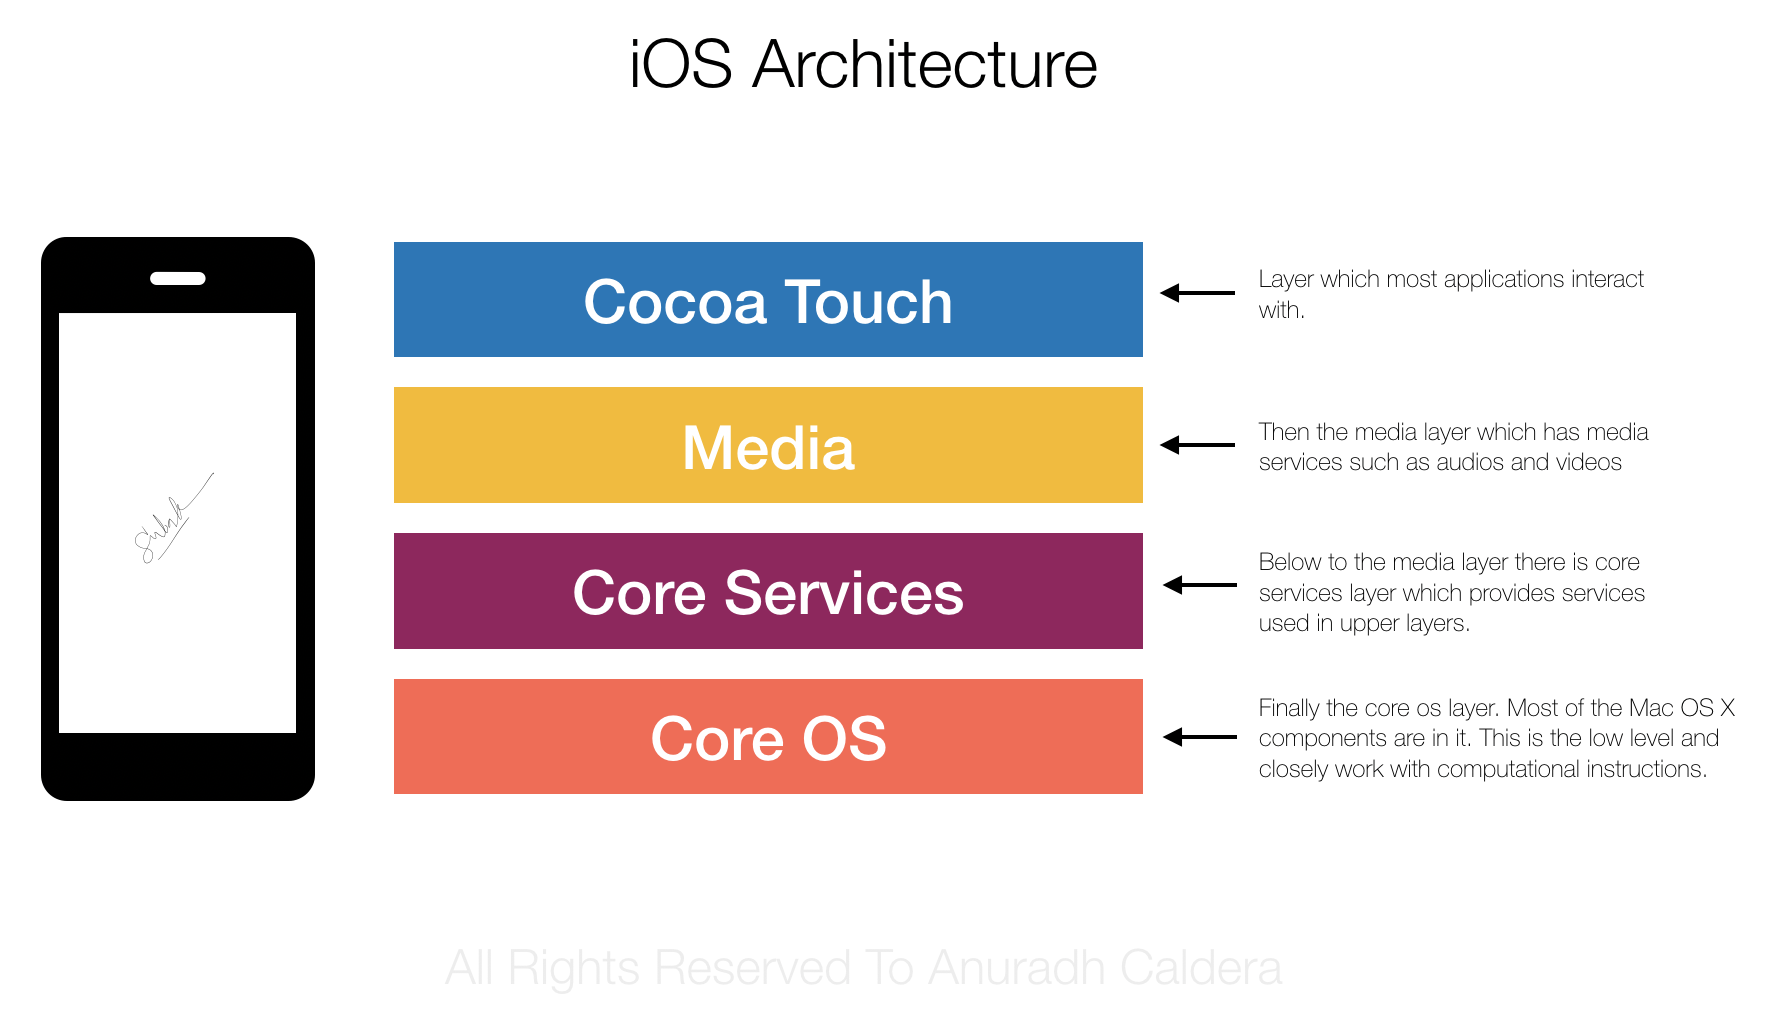
\includegraphics[width=6in]{images/Chapitre1/ios_architecture.png}
    \label{fig:ios Ui}
    \caption{L'architecture de iOS}
\end{figure}

\newpage
\section{Les applications mobiles}
\subsection{Definition}
Une application mobile est un logiciel installable sur les appareils mobile par exemple une tablette tactile ou un smartphone, pour but d'exécuter des tâches spécifiques.

La plupart des applications mobiles sont distribuées au public par le biais de plateformes de téléchargement généralement gérée par les fabricants de appareils mobiles comme Google Play Store par Android/Google ou encore App Store pour les produits Apple. Ces applications sont disponibles soit en version gratuite et qui contient généralement des publicités soit en version payante.

Sur certaines plateformes, les applications peuvent aussi être installées à partir de sources tierces, via un site non affilié au distributeur d'origine. Sur Android, cela est possible en activant le mode développeur. Sur iOS, cette manipulation est possible soit en étant développeur Apple, soit en possédant un appareil jailbreaké.~\cite{ApplicationMobile2020}

les applications mobiles se regroupent en plusieurs séries, on trouve : 
\begin{itemize}
   \item Les jeux mobiles.
   \item Les applications a but éducatif.
   \item Les applications de géolocalisation.
   \item Les applicatopns d'écoute de musiques ou de radios et de streaming vidéo.
   \item Les applications pour la consultation d'Internet.
   \item Les applications des réseaux sociaux.
\end{itemize}

\begin{figure}[!ht]
    \centering
    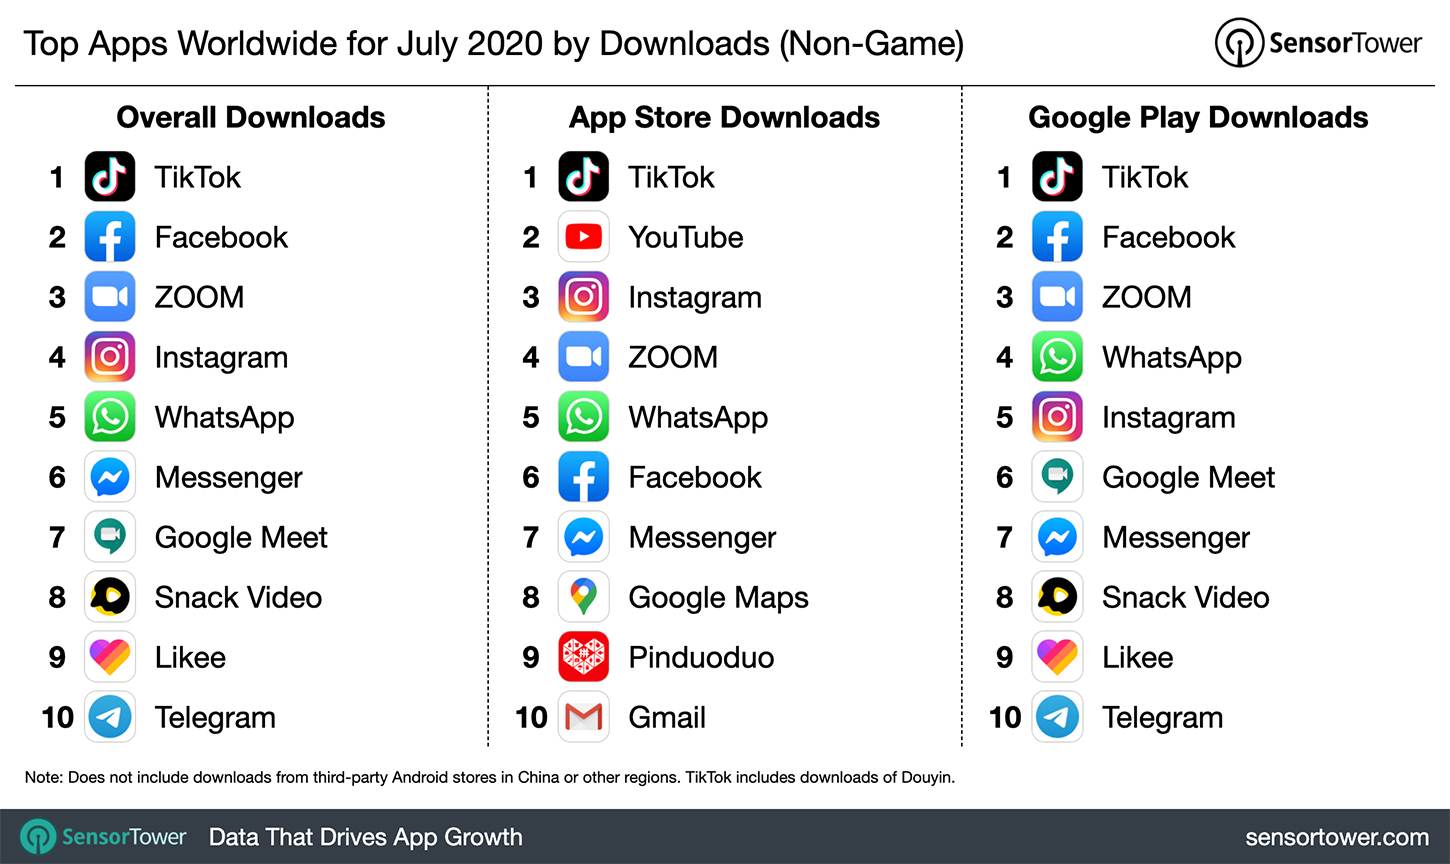
\includegraphics[width=4.6in]{images/Chapitre1/app_downloads.jpg}
    \label{fig:ios Ui}
    \caption{Classement des meilleures applications dans le monde pour juillet 2020 par téléchargements}
\end{figure}
\newpage
\subsection{Les types des applications mobiles}
Il existe dans le domaine des applications mobiles trois types d'applications en parlant du language de programmation et les taches que fait l'application. On trouve donc :
\subsubsection{Application native :}
Les applications natives sont des applications conçues spécialement pour les systèmes d'exploitation fiables par les smartphones. Ces applications utilisent chaqune un language de programmation spéciale pour chaque système d'exploitation, comme Java pour Android et Swift pour iOS.
\subsubsection{Application web :}
Une application web est une application conçue avec le language HTML et CSS, ce type d'application fonctionne de manière flexible sur tous les navigateurs internet dans les appareils mobiles. 
\subsubsection{Application hybride :}
Les applications hybrides regroupent les caractéristiques des applications web et applications mobilent, elles sont donc accessibles via toutes les plateformes des applications. ce type d'application réduit la durée et les charges du développement.


\begin{figure}[!ht]
    \centering
    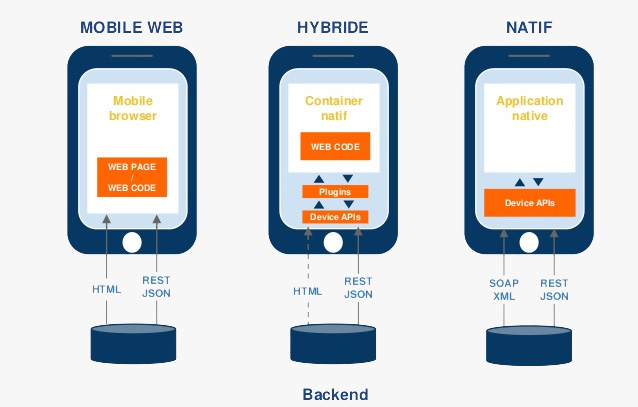
\includegraphics[width=6in]{images/Chapitre1/type_applications_mobile.jpg}
    \label{fig:type_applications}
    \caption{Les trois types d'applications mobile}
\end{figure}
\subsection{Le cycle de vie d'une application mobile}
Le cycle de vie d'une application mobile se compose de 6 phases de travail ~\cite{CycleVieDeveloppement}, citons-les:
     
\subsubsection{1- Planification et analyse:}
La première étape de la conception consiste à analyser la situation pour tenir compte des contraintes, des risques et de tout autre élément pertinent et assurer un ouvrage ou un processus répondant aux besoins du client.
\subsubsection{2- Spécification technique:}
Dans cette étape, On détermine le type des opérations ainsi que les systèmes pour lesquels on souhaite créer l'application mobile. On établit à la fin un cahier de charge.

\subsubsection{3- Prototypage et conception:}
À cette étape, des diagrammes UML ainsi que des diagrammes d'action sont créé puis on crée un prototype de l'application qui aide le client pour valider l'idée et commencer la phase suivante
\subsubsection{4- Développement:}
Le processus de développement d'applications est divisé en deux phases : front-end et backend. Cette étape consiste à coder les modules de l'application un par un et effectuer des tests sur place avant d'entamer le prochain module. Cependant, le développement de la partie backend n'est pas toujours nécessaire si on utilise des techniques cloud pour le traitement et le stockage des données 
\subsubsection{5- Tests et assurance de qualité:}
La phase de tests et assurance de qualité est une partie très importante pour la création de l'application. cette phase comprend des tests des exigences, interfaces et de la sécurité de l'application et des données ainsi que les ressources du bas niveau.
\subsubsection{6- Maintenance et mise à jour:}
Après la phase de tests,on est dans la phase finale où l'application est prête pour la distribution dans les plateformes d'achat des applications, mais le travail ne s'arrête pas là, l'application doit être mise à jour de façon reguiliére pour répondre aux nouveaux besoins des utilisateurs. 


 %  \newcommand\tab[1][0,4cm]{\hspace*{#1}}
\newcommand\longtab[1][1cm]{\hspace*{#1}}

\chapter{Les technologies utilisées}
\section{Introduction}
Ces dernières années, le secteur du développement des applications mobiles a connu une majeure évolution avec l’apparition des outils de développement cross-platform. Ces outils permettent la création d’une application mobile avec une base de code unique sur les différents environnements Ios et Android. 

Au cours de ce chapitre nous allons nous présenterons d'abbord Flutter, un des frameworks utilisés pour le développement des applications multiplate-forme, ensuite nous allons parler de Firebase,  un service Google utilisé dans le côté Backend des applications. Pour finaliser nous allons définir les api Google ainsi que google maps.
\section{Flutter}
\begin{wrapfigure}[8]{r}{2cm}
    \vspace{-15pt}
    
\includegraphics[width=2cm]{images/flutterLogo.png}
    \vspace{-15pt}
\caption{{\footnotesize Logo de Flutter}}
\end{wrapfigure}
Flutter est un SDK d'application permettant de créer des applications haute performance et haute fidélité pour ios, Android, Web (version bêta) et de bureau (aperçu technique) à partir d'une base de code unique.~\cite{TechnicalOverview}
L'objectif est de permettre aux développeurs de fournir des applications hautes performances qui semblent naturelles sur différentes plateformes notamment appelés les applications multi-platformes.
\\
Flutter s’appuie sur le langage de programmation DART (à l’origine appelé Dash), créé également par Google et présenté au public en 2011.

Les applications Flutter s’exécutent dans une machine virtuelle, cette dernière offre une fonctionnalité du rechargement rapide de l’application sans avoir besoin de recompiler le projet, les applications sont donc compilées directement en code machine, sois en Javascript si elles sont destinées au web ou en instructions Intel X64 ou ARM. 
\newpage
Le framework Flutter est open source, avec une licence BSD permissive, et dispose d'un écosystème florissant de packages tiers qui complètent les fonctionnalités de base de la bibliothèque.
\begin{figure}[!h]

    \centering
    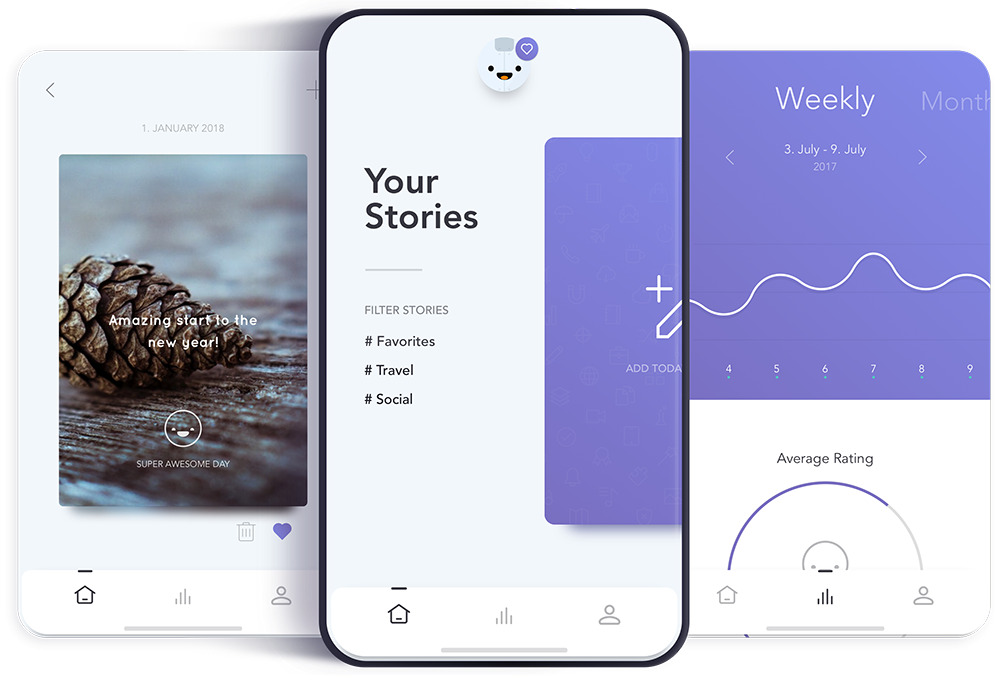
\includegraphics[width=3in]{images/Chapitre2/reflectly_app.png}
    \label{fig:firebasepricing}
    \caption{Exemple de l'application Reflectly développée avec le framework Flutter}
\end{figure}

Flutter est conçu comme un système extensible en couches. Il existe sous la forme d'une série de bibliothèques indépendantes qui dépendent chacune de la couche sous-jacente. Aucune couche n'a un accès privilégié à la couche ci-dessous, et chaque partie du niveau de structure est conçue pour être facultative et remplaçable.~\cite{FlutterArchitecturalOverview}

\begin{figure}[!h]

    \centering
    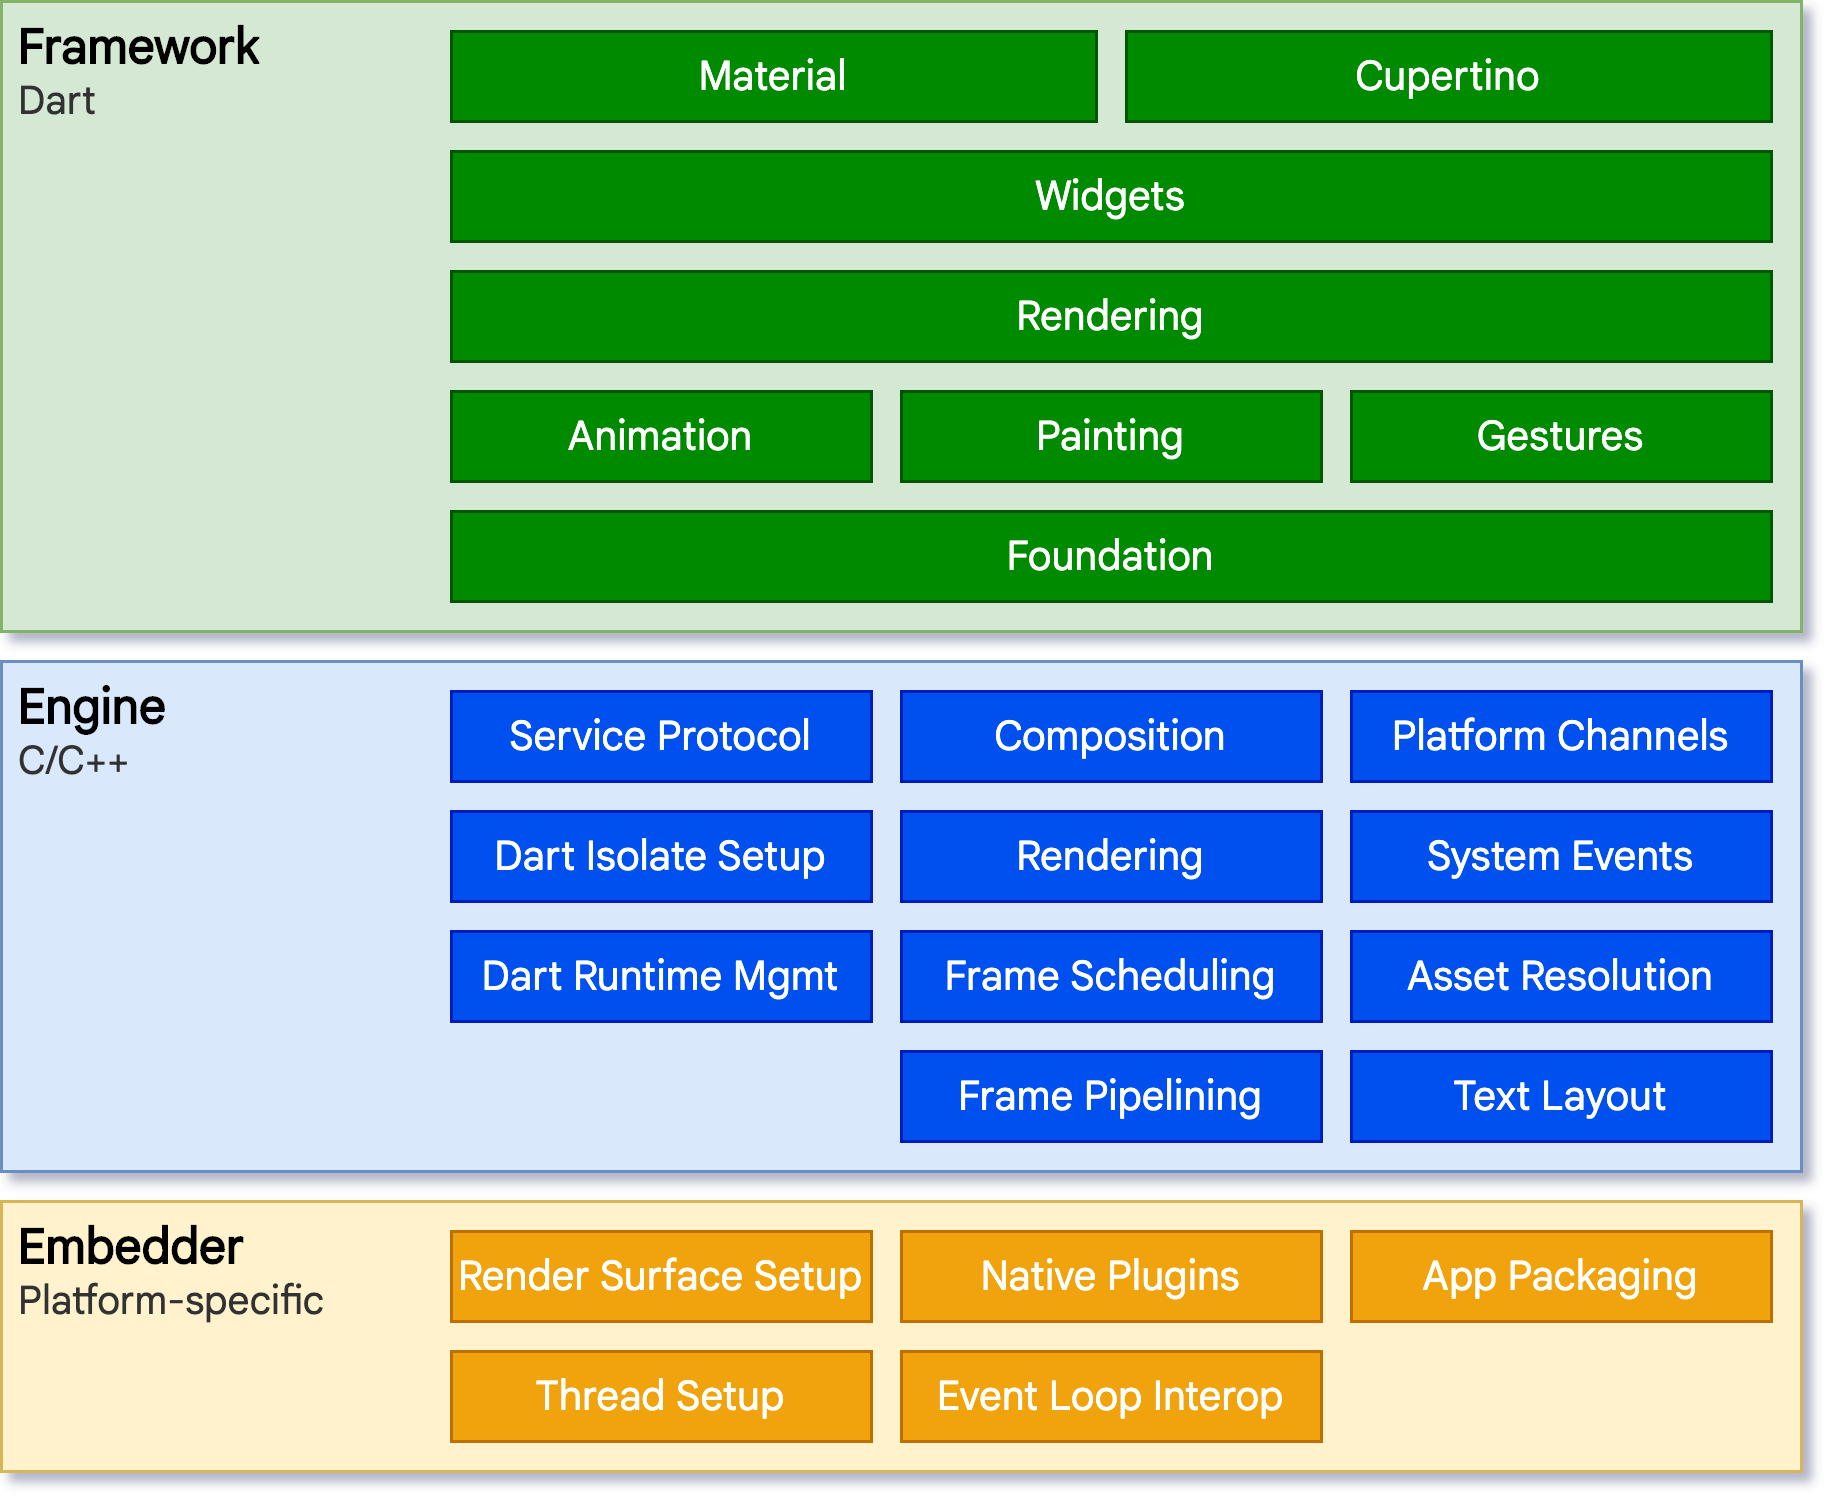
\includegraphics[width=5in]{images/Chapitre2/flutter_architectures.png}
    \label{fig:firebasepricing}
    \caption{L'architecutre du framework Flutter}
\end{figure}

\newpage


\newpage
\subsection{Principes de base}
Flutter comprend un framework de style react moderne, un moteur de rendu 2D, des widgets prêts à l’emploi et des outils de développement. Ces composants fonctionnent ensemble pour vous aider à concevoir, créer, tester et déboguer des applications.Tout est organisé autour de quelques principes fondamentaux.
\begin{enumerate}
    \item \textbf{Tout est un widget: }\\
          Les widgets sont les éléments de base de l’interface utilisateur d’une application Flutter. Chaque widget est une déclaration immuable d’une partie de l’interface utilisateur. Contrairement aux autres frameworks qui séparent les vues, les contrôleurs de vue, les présentations et d’autres propriétés, Flutter possède un modèle objet cohérent et unifié : le widget. Un widget peut
          définir :
          \begin{itemize}
              \item un élement structurel (comme un bouton ou un menu).
              \item un élement stylistique (comme une police ou un jeu de couleurs).
              \item un aspect de la mise en page (comme le rembourage).
              \item etc...
          \end{itemize} 
          
          \item \textbf{L'utilisation du language Dart}\\
       
        Le Dart est un langage de programmation structuré, open source et évolutif qui fonctionne à l'aide d'une machine virtuelle. Le projet de google à travers le Dart est de faciliter le développement web, de combler les carences du Javascript et d'offrir de meilleures performances, surtout pour les gros projets. Le Dart est destiné à fonctionner sur les navigateurs web modernes ainsi que sur les serveurs et il embarque également un convertisseur Javascript. Il y a plusieurs manières d'exécuter du code Dart; soit en utilisant un navigateur qui supporte directement ce code, soit en le compilant. En plus du navigateur Web et de la convertion javascript, le code peut être exécuté en ligne de commande, hébergé dans une machine virtuelle ce qui permet au client et au serveur d'avoir les applications écrites dans le même langage.~\cite{DartSUPINFOEcole}\bigskip
          \item \textbf{Hot Reload: }\\ 
          La fonctionnalité Hot Reload fonctionne en injectant des fichiers de code source mis à jour dans la machine virtuelle Dart (VM) en cours d'exécution. Une fois que la machine virtuelle a mis à jour les classes avec les nouvelles versions de champs et de fonctions, le framework Flutter reconstruit automatiquement l'arborescence des widgets, vous permettant de visualiser rapidement les effets de vos modifications. le build des applications est très rapide, ce qui rend quasiment invisible le temps de compilation. Un gain de temps pour les développeurs .
        \end{enumerate}          
\newpage

\subsection{Pourquoi utiliser flutter ?  }           
\textbf{-Multi-plateforme (Cross-platform)}\\
Flutter permet d'avoir une seule base de code pour tous les systèmes d'exploitation choisis. Puisque tout dans Flutter est un widget, le code est un balisage.\bigskip

\textbf{-Compatibilité avec toutes les version Android/iOS}\\
La prise en charge des applications mobiles par tous les appareils et toutes les versions du système d'exploitation est devenue un gros problème.

Ce problème a été résolu par Flutter qui a son propre moteur et des widgets pris en charge à la fois par les composants matériels pour android et Cupertino pour IOS. Les applications développées avec flutter sons prise en charge depuis la version IOS 8 et Android jelly Bean jusqu'à la dernière version.\bigskip

\textbf{-Performance et stabilité}\\
Le code de Flutter est compilé dans le code ARM du processeur. Avec son propre moteur de rendu, les applications Flutter ne sont affectées par aucune mise à jour du système d'exploitation ou personnalisation du système. Ils auront toujours la même apparence en termes d'interface même après une mise à jour du système iOS ou Android.

La compatibilité des versions est un autre aspect de l'influence de la stabilité. En tant que boîte à outils en croissance rapide, Flutter ne change pas son API et ses approches de développement. Le code écrit il y a deux ans pourrait être réutilisé dans les applications nouvellement créées.
\bigskip

% \textbf{-Productivité}\\
% Flutter offre une augmentation de la productivité qui provient
% du rechargement a chaud. Cela permet aux développeurs de voir les modifications apportée à l'état de l'application en un temps record.
 
\newpage
\section{Firebase}
\begin{wrapfigure}[8]{r}{3cm}
    \vspace{-15pt}
    
\includegraphics[width=3cm]{images/Chapitre2/firebase_logo.png}
    \vspace{-20pt}
    \caption{{\footnotesize Logo de Firebase}}
\end{wrapfigure}
Firebase est un ensemble de services d'hébergement pour n'importe quel type d'application, il propose d'héberger en NoSQL et en temps réel des bases de données,
du contenu, de l'authentification sociale (Google, Facebook, Twitter et Github),
et des notifications, ou encore des services, tel que par exemple un serveur
de communication temps réel.~\cite{Firebase2020}
\subsection{Les services de Firebase}
La platforme Firebase peut fournir trois types de services:\bigskip

\tab \textbf{1 - Construction des meilleures applications:}\bigskip

\begin{wrapfigure}[3]{l}{1cm}
 	
\includegraphics[width=1cm]{images/Chapitre2/Firebase_services/firestore.PNG}
 \end{wrapfigure}
\textbf{Cloud Firestore} Permet de stocker et synchroniser les données entre utilisateurs et appareils - à l’échelle mondiale - à l’aide d’une base de données NoSQL hébergée dans le cloud. Cloud Firestore offre donc
une synchronisation en direct et une assistance hors ligne, ainsi que
des requêtes de données efficaces. Son intégration avec d’autres produits Fi-
rebase permet de créer de véritables applications sans serveur.\medskip

\begin{wrapfigure}[3]{l}{1cm}
	
\includegraphics[width=1cm]{images/Chapitre2/Firebase_services/mlkit.PNG}
\end{wrapfigure}
\textbf{Kit ML \textsuperscript{BETA}} Ce service Apporte de puissantes fonctionnalités
d'apprentissage automatique au applications mobile. Firebase ML aide
à déployer des modèles ML personnalisés optimisés pour l'inférence sur
l'appareil, ce qui réduit la taille d'installation initiale de
l'application et permet d'effectuer plus facilement des mises à jour.
on peut également utiliser AutoML Vision Edge pour entraîner nos
propres modèles de classification d'images personnalisés ou accéder aux
API Cloud AI Vision pour une solution plus clé en main.\medskip

\begin{wrapfigure}[4]{l}{1cm}
	
\includegraphics[width=1cm]{images/Chapitre2/Firebase_services/cloud_function.PNG}
\end{wrapfigure}
\textbf{Fonctions cloud} Grace a ce service on peut devlopper les applications avec
un code backend personnalisé
sans avoir à gérer et à mettre à l'échelle nos propres serveurs.
Les fonctions peuvent être déclenchées par des événements, qui sont
émis par les produits Firebase, les services Google Cloud ou des tiers,
à l'aide de webhooks.\medskip

\begin{wrapfigure}[4]{l}{1cm}
	
\includegraphics[width=1cm]{images/Chapitre2/Firebase_services/authentication.PNG}
\end{wrapfigure}
\textbf{Authentification} Ce service permer de gérer les utilisateurs de manière simple et sécurisée.
Firebase Auth propose plusieurs méthodes pour s'authentifier,
y compris l'e-mail et le mot de passe, des fournisseurs tiers
comme Google ou Facebook, et en utilisant directement le
système de compte existant.\medskip

\begin{wrapfigure}[4]{l}{1cm}
	
\includegraphics[width=1cm]{images/Chapitre2/Firebase_services/hosting.PNG}
\end{wrapfigure}
\textbf{Hebergement} Avec ce service Firebase , l'hébergement est facile avec grace outils spécialement
conçus pour les applications Web modernes. Lorsqu'on telecharge nos
ressources Web, ces dernieres sont automatiquement transferées vers le  CDN mondial
et leur fournissons un certificat SSL gratuit afin que les utilisateurs de l'application
bénéficient d'une expérience sécurisée, fiable et à faible latence, où qu'ils se trouvent.\medskip

\begin{wrapfigure}[4]{l}{1cm}

\includegraphics[width=1cm]{images/Chapitre2/Firebase_services/cloud_storage.PNG}
\end{wrapfigure}
\textbf{Stockage en ligne} Grace a Firebase on peut Stocker et partager du contenu généré par les utilisateurs de notre application,
comme des images, de l'audio et de la vidéo avec un stockage d'objets puissant,
simple et économique conçu pour l'échelle de Google. Les SDK Firebase pour Cloud
Storage ajoutent la sécurité de Google aux importations et aux téléchargements de
fichiers pour nos applications Firebase, quelle que soit la qualité du réseau.\medskip

\begin{wrapfigure}[4]{l}{1cm}
    
\includegraphics[width=1cm]{images/Chapitre2/Firebase_services/realtime_database.PNG}
    \end{wrapfigure}
\textbf{Base de données en temps réel} Realtime Database est la base de données originale
de Firebase. C'est une solution efficace et à faible latence pour les applications
mobiles qui nécessitent des états synchronisés entre les clients en temps réel.
Le service Cloud Firestore est fortement recommendé au lieu de Realtime Database pour la plupart
des développeurs qui démarrent un nouveau projet.\bigskip

\tab \textbf{2 - Amelioaration de la qualité des applications:}\bigskip

\begin{wrapfigure}[4]{l}{1cm}
    
\includegraphics[width=1cm]{images/Chapitre2/Firebase_services/crashlytics.PNG}
    \end{wrapfigure}
\textbf{Crashlytics} Permet de réduire le temps de dépannage en transformant une avalanche
de plantages en une liste gérable de problémes. On obtien donc des informations claires et exploitable 
sur les problèmes à résoudre en premier en voyant l'impact de l'utilisateur directement dans le tableau
 de bord Crashlytics. Crashlytics est donc le principal reporter de crash de Firebase.\medskip

\begin{wrapfigure}[4]{l}{1cm}

\includegraphics[width=1cm]{images/Chapitre2/Firebase_services/performance_monitoring.PNG}
    \end{wrapfigure}
\textbf{Suivi des performances} Grace a ce service on peut diagnostiquer les problèmes de performances 
des applications survenant sur les appareils de nos utilisateurs. Donc on peut rester au courant 
de l'heure de démarrage de notre application et surveiller les requêtes HTTP sans écrire de code.\medskip

\begin{wrapfigure}[4]{l}{1cm}
    
\includegraphics[width=1cm]{images/Chapitre2/Firebase_services/test_lab.PNG}
        \end{wrapfigure}
\textbf{Laboratoire de test} Avec ce service on peut executer des tests automatiques et personnalisés pour 
notre application sur des appareils virtuels et physiques hébergés par Google.On peut alors decouvrir 
tout les bugs et les incoherences afin de pouvoir ofirir une excellent expérience au utilisateurs 
sur un large choix d'appareils .\medskip
 
\begin{wrapfigure}[4]{l}{1cm}
    
\includegraphics[width=1cm]{images/Chapitre2/Firebase_services/App_distribution.jpg}
        \end{wrapfigure}
\textbf{Distribution d'applications \textsuperscript{BETA}} Firebase App Distribution permet aux développeurs
 d'envoyer des versions préliminaires de leur application à des testeurs de confiance à partir de la console 
 ou à l'aide d'outils de ligne de commande, ainsi que de gérer les testeurs en un seul endroit.\bigskip 

\tab \textbf{3 - Developpement de l'entreprise:}\bigskip


\begin{wrapfigure}[4]{l}{1cm}
    
\includegraphics[width=1cm]{images/Chapitre2/Firebase_services/in-app_messaging.PNG}
        \end{wrapfigure}
\textbf{Messagerie integrée a l'application \textsuperscript{BETA}} Donne le pouvoir de déclencher 
des messages en fonction du comportement et des intérêts des utilisateurs. On peut aussi personnaliser
la conception des messages intégrés à l'application en fonction de notre marque. La messagerie 
intégrée prend en charge une variété de cas d'utilisation et de formats. \medskip 

\begin{wrapfigure}[4]{l}{1cm}
    
\includegraphics[width=1cm]{images/Chapitre2/Firebase_services/google_analytics.PNG}
        \end{wrapfigure}
\textbf{Google analytics} Grace aux informations en temps réel à partir de rapports on peut
Analyser les attributions et le comportement des utilisateurs et aussi exporter nos données
d'événement brutes vers Google BigQuery pour une analyse personnalisée. \medskip 

\begin{wrapfigure}[4]{l}{1cm}
    
\includegraphics[width=1cm]{images/Chapitre2/Firebase_services/a_b_testing.PNG}
        \end{wrapfigure}
\textbf{Tests A/B} L'exécution des expériences produit et marketing nous permet d'ameliorer
des tests A / B . Grace a ce service on peut personnaliser les tests en fonction de nos
objectifs et tester diverses mises à jour de notre application, comme la copie de messages
ou de nouvelles fonctionnalités. \medskip 

\begin{wrapfigure}[4]{l}{1cm}
    
\includegraphics[width=1cm]{images/Chapitre2/Firebase_services/predictions.PNG}
        \end{wrapfigure}
\textbf{Prédictions} La puissance de l'apprentissage automatique de Google est exploitée
par ce service pour obtenir des informations sur les segments d'utilisateurs susceptibles
de générer des revenus ou de dépenser (ou de terminer un autre événement de conversion).
Ces segments prédictifs intelligents peuvent etre utilisés pour cibler d'autres produits
tels que Remote Config, Cloud Messaging et In-App Messaging.\medskip 

\begin{wrapfigure}[4]{l}{1cm}
    
\includegraphics[width=1cm]{images/Chapitre2/Firebase_services/cloud_messaging.PNG}
        \end{wrapfigure}
\textbf{Messagerie Cloud} Grace a ce service on peut envoyer gratuitement des messages
et des notifications aux utilisateurs sur toutes les plates-formes (Android, iOS et 
le Web). Les messages peuvent être envoyés à des appareils uniques, à des groupes 
d'appareils ou à des sujets ou segments d'utilisateurs spécifiques. Firebase Cloud Messaging
(FCM) s'adapte même aux applications les plus volumineuses, fournissant des centaines de
milliards de messages par jour. \medskip 

\begin{wrapfigure}[4]{l}{1cm}
    
\includegraphics[width=1cm]{images/Chapitre2/Firebase_services/remote_config.PNG}
        \end{wrapfigure}
\textbf{Configuration a distance} Grace a ce service on peut personnaliser le rendu de
votre application pour chaque utilisateur, Modifier l'apparence, déployer les 
fonctionnalités progressivement, exécuter des tests A / B, fournir du contenu personnalisé
à certains utilisateurs ou effectuer d'autres mises à jour sans déployer une nouvelle
version.On peut aussi surveiller l'impact des modifications et effectuer des ajustements
en quelques minutes.\medskip 

\begin{wrapfigure}[4]{l}{1cm}
    
\includegraphics[width=1cm]{images/Chapitre2/Firebase_services/dynamic_links.PNG}
        \end{wrapfigure}
\textbf{Liens dynamiques} L'utilisation des liens dynamiques offre une expérience utilisateur
personnalisée pour iOS, Android et le Web. On les utiliser pour alimenter le Web mobile afin
de générer des conversions d'applications natives, un partage d'utilisateur à utilisateur,
des campagnes sociales et marketing, etc. Les liens dynamiques fournissent les attributions
dont on a besoin pour mieux comprendre notre croissance mobile.\medskip 
\subsection{Pourquoi utiliser Firebase ?}
Sachant que la majorité des la communité des developpeurs considére Firebase comme le Meilleur 
service BaaS (backend as a service) et l'utilise dans la majorité de leurs projets , il existe 
d'autre alternatives , parmi les alternatives on a : 

- La construction manuelle du service de gestion de l'infrastructure Backend de notre application.

\textbf{Parse :}\medskip
\begin{wrapfigure}[8]{r}{2cm}
    \vspace{-15pt}
    
\includegraphics[width=2cm]{images/Chapitre2/parse_logo.png}
    \vspace{-20pt}
    \caption{{\footnotesize Logo de Parse}}
\end{wrapfigure}
Parse est un service BaaS développé par Facebook. Parse
est un serveur Open Source, il offre donc un controle total
du code et on peut ajouter nos propre fonctions et elements. Cepandant 
l'implementation du service dans l'application reste tres difficile .

- Il existe autre alternatives comme Back4App, Backendless,
Kinvey, AWS Amplify, etc.


Cepandant, On a trouvé que Firebase est la meilleure solution a utiliser
pour notre projet pour les raisons suivantes : 

- La documentation est assez solide contrairement a parse et les autres alternatives.

- La facilité d'implementation des services d'authentification comme Google, Facebook et Github.

- La facilité de l'integration avec Flutter car Flutter et Firebase travaillent main dans la main
 pour nous aider à créer des applications mobiles en un temps record.

- La flexibilité de la tarification des services Firebase. On peut commencer gratuitement,
puis on paye au fur et à mesure celon nos besoins.~\cite{FirebasePricing}
\begin{figure}[!h]

    \centering
    
\includegraphics[width=6in]{images/Chapitre2/firebase_pricing_offers.PNG}
    \label{fig:firebasepricing}
    \caption{Exemple de la tarification d'une partie des services Firebase}
\end{figure}

\newpage

\section{Google APIs}

Les API Google sont des interfaces de programmation d'application
( API ) développées par Google qui permettent la communication avec
les services Google et leur intégration à d'autres services. Les exemples
de ceux-ci incluent la recherche, Gmail, la traduction ou Google Maps.
Les applications tierces peuvent utiliser ces API pour tirer parti ou
étendre les fonctionnalités des services existants.

Les API fournissent des fonctionnalités telles que l'analyse,
l'apprentissage automatique en tant que service (l'API de prédiction)
ou l'accès aux données utilisateur (lorsque l'autorisation de lire les
données est donnée). Un autre exemple important est une carte Google intégrée
sur un site Web, qui peut être réalisée à l'aide de l'API Static Maps,
Places API ou de l'API Google Earth .~\cite{GoogleAPIs2020}
\\
\begin{figure}[!h]

    \centering
    
\includegraphics[width=4in]{images/Chapitre2/GoogleAPIs.jpeg}
    \label{fig:googleapis}
    \caption{Logo de Google APIs}
\end{figure}
\\
Dans ce projet nous avons utilisé deux APIs : Google Maps et Google Places dont
on va en parler dans la section suivante.
\subsection{Google Maps}
Google Maps est un ervice de cartographie web,ce service disponible sur ordinateur, tablette et smartphone qui permet, à partir de l'échelle mondiale, de zoomer jusqu'à l'échelle d'une habitation.
Plusieurs types de vue sont
disponibles dans Google Maps :
une vue en plan cartographique classique,
avec les noms des rues, quartiers, villes et
une vue en images satellites ou photographies
aériennes, qui couvre aujourd'hui le monde
entier, une vue en images obliques couvrant
les grandes villes du monde et certaines
villes secondaires et une vue avec le relief.~\cite{GoogleMapsWikipedia}

Avec le SDK Maps pour Android, on peut ajouter des cartes basées
sur les données de Google Maps à notre application.
L'API gère automatiquement l'accès aux serveurs Google Maps, le
téléchargement des données, l'affichage de la carte et la réponse aux
gestes de la carte. On peut également utiliser les appels d'API pour
ajouter des marqueurs, des polygones et des superpositions à une carte de
base et pour modifier la vue de l'utilisateur d'une zone de carte
particulière. Ces objets fournissent des informations supplémentaires
sur les emplacements de la carte et permettent à l'utilisateur d'interagir
avec la carte.
\\
L'API nous permet d'ajouter ces graphiques à une carte:
\begin{itemize}
    \item Icônes ancrées à des positions spécifiques sur la carte (marqueurs).
    \item Ensembles de segments de ligne (polylignes).
    \item Segments fermés (polygones).
    \item Graphiques bitmap ancrés à des positions spécifiques sur la carte (superpositions au sol).
    \item Ensembles d'images qui sont affichés au-dessus des tuiles de la carte de base.
\end{itemize}
\begin{figure}[!h]

    \centering
    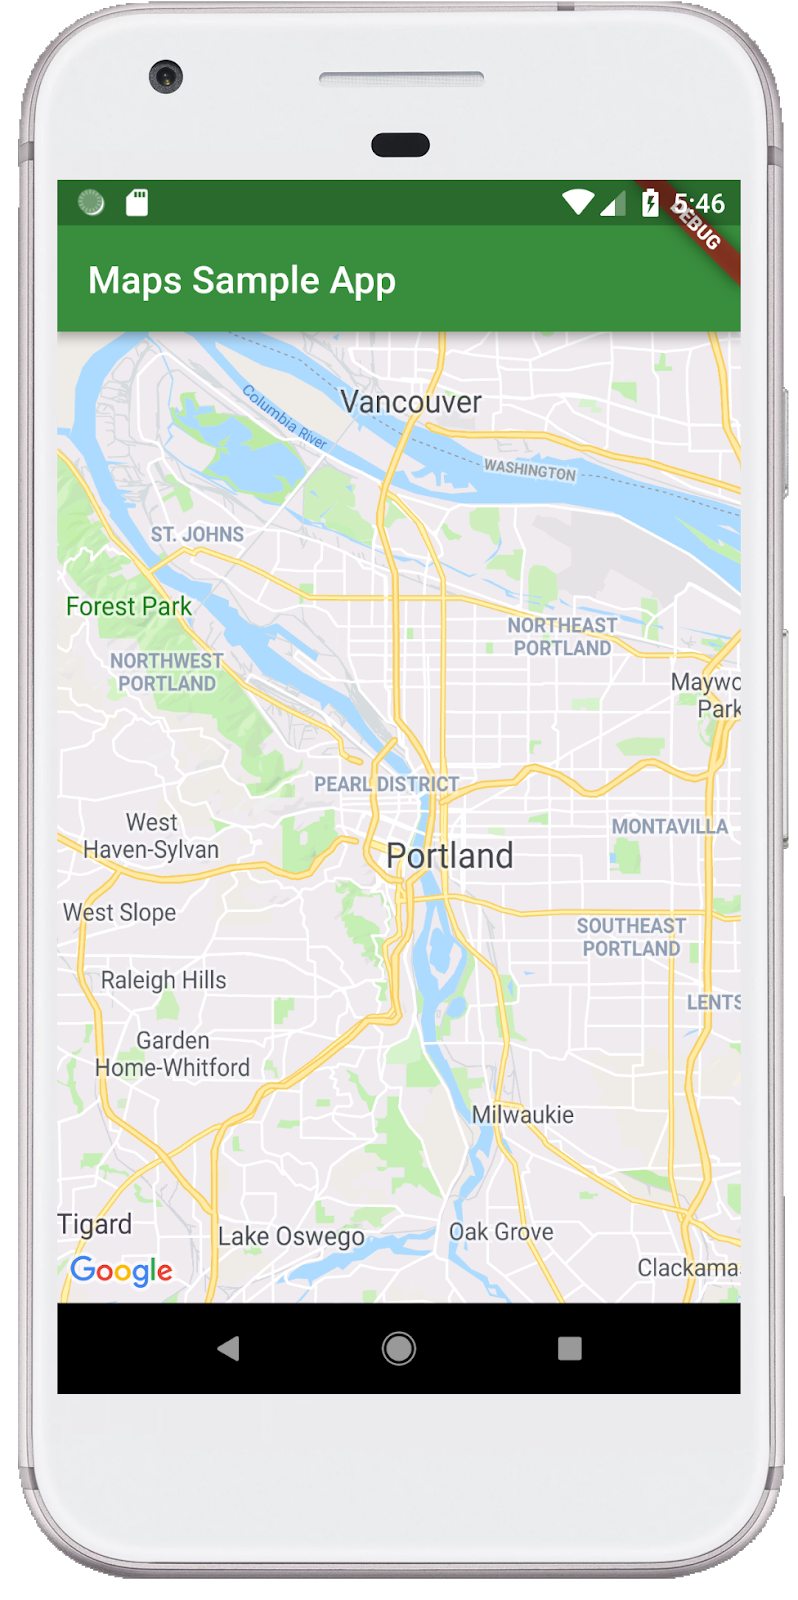
\includegraphics[width=2in]{images/Chapitre2/GoogleMapsMobile.png}
    \label{fig:GoogleMapsMobile}
    \caption{Exemple de l'integration des services Google Maps dans une application mobile}
\end{figure}


\chapter{Conception et implémentation de l'application}
\section{Introduction}
Après avoir étudié les différents techniques utilisés pour le développement des applications mobiles, on va entamer dans ce chapitre la partie conception et implémentation de notre application Android en fixant les objectifs de cette application suivie par une étude comparative sur des solutions déjà existantes, ensuite on va présenter les diagrammes UML ainsi que le diagramme d'action, puis les maquettes fonctionnelles et les interfaces utilisateur. À la fin on termine avec les outils matériels et logiciels utilisés au long du cursus du développement de l’application.
\section{Conception}
\subsection{Objectif du projet}
Ce projet a pour but de développer une application mobile sous la plateforme Android. qui permettra d'afficher dans une carte géographique des restaurants qui sont à proximité de l'utilisateur avec les informations de ces derniers ainsi que les menus qui lui seront accessible tous ça a pour but de rendre la recherche sur les restaurants et les menus plus facile et efficace .
\subsection{Applications déja existantes}
\paragraph*{}
Il existe peu d'applications mobiles dans le domaine de la restauration nous allons explorer certaines des plus populaires solutions existantes aujourd’hui.

\newpage
\subsubsection{TripAdvisor}
\begin{wrapfigure}[8]{r}{2cm}
    \vspace{-15pt}
    
\includegraphics[width=2cm]{images/Chapitre1/tripadvisor.png}
    \vspace{-20pt}
    \caption{{\footnotesize Logo de TripAdvisor}}
\end{wrapfigure}

TripAdvisor est une plate-forme disponible en web et en application mobile, cette plate-forme offre des avis et des suggestions d'hôtels, lieux de loisirs, villes et régions à l'échelle internationale, compare les prix et affiche les meilleures offres du moment.

TripAdvisor couvre aussi les services de restauration et fournit des informations sur les différents restaurants qui existent dans le monde entier. \bigskip

Le service qu'offre cette plate-forme pour le secteur de la restauration a des avantages : \bigskip

	\tab- L'utilisation de ce service est gratuite.\medskip

	\tab- Donne un aperçu sur les restaurants et offre des informations sur la fourchette des prix..\medskip

	\tab- Des évaluations et des avis sont fournis par les utilisateurs eux-mêmes.\bigskip

TripAdvisor a ses avantages mais aussi ses inconvénients:\bigskip

	\tab- On ne peut pas parcourir les restaurants en utilisant une carte géographique.\medskip

	\tab- L'utilisation d'une application tierce est indispensable pour avoir l'itinéraire vers les restaurants.\medskip

	\tab- Les informations offertes par cette plate-forme sont limitées au avis fourni par les utilisateurs.
 

	\begin{figure}[!ht]

		\centering
		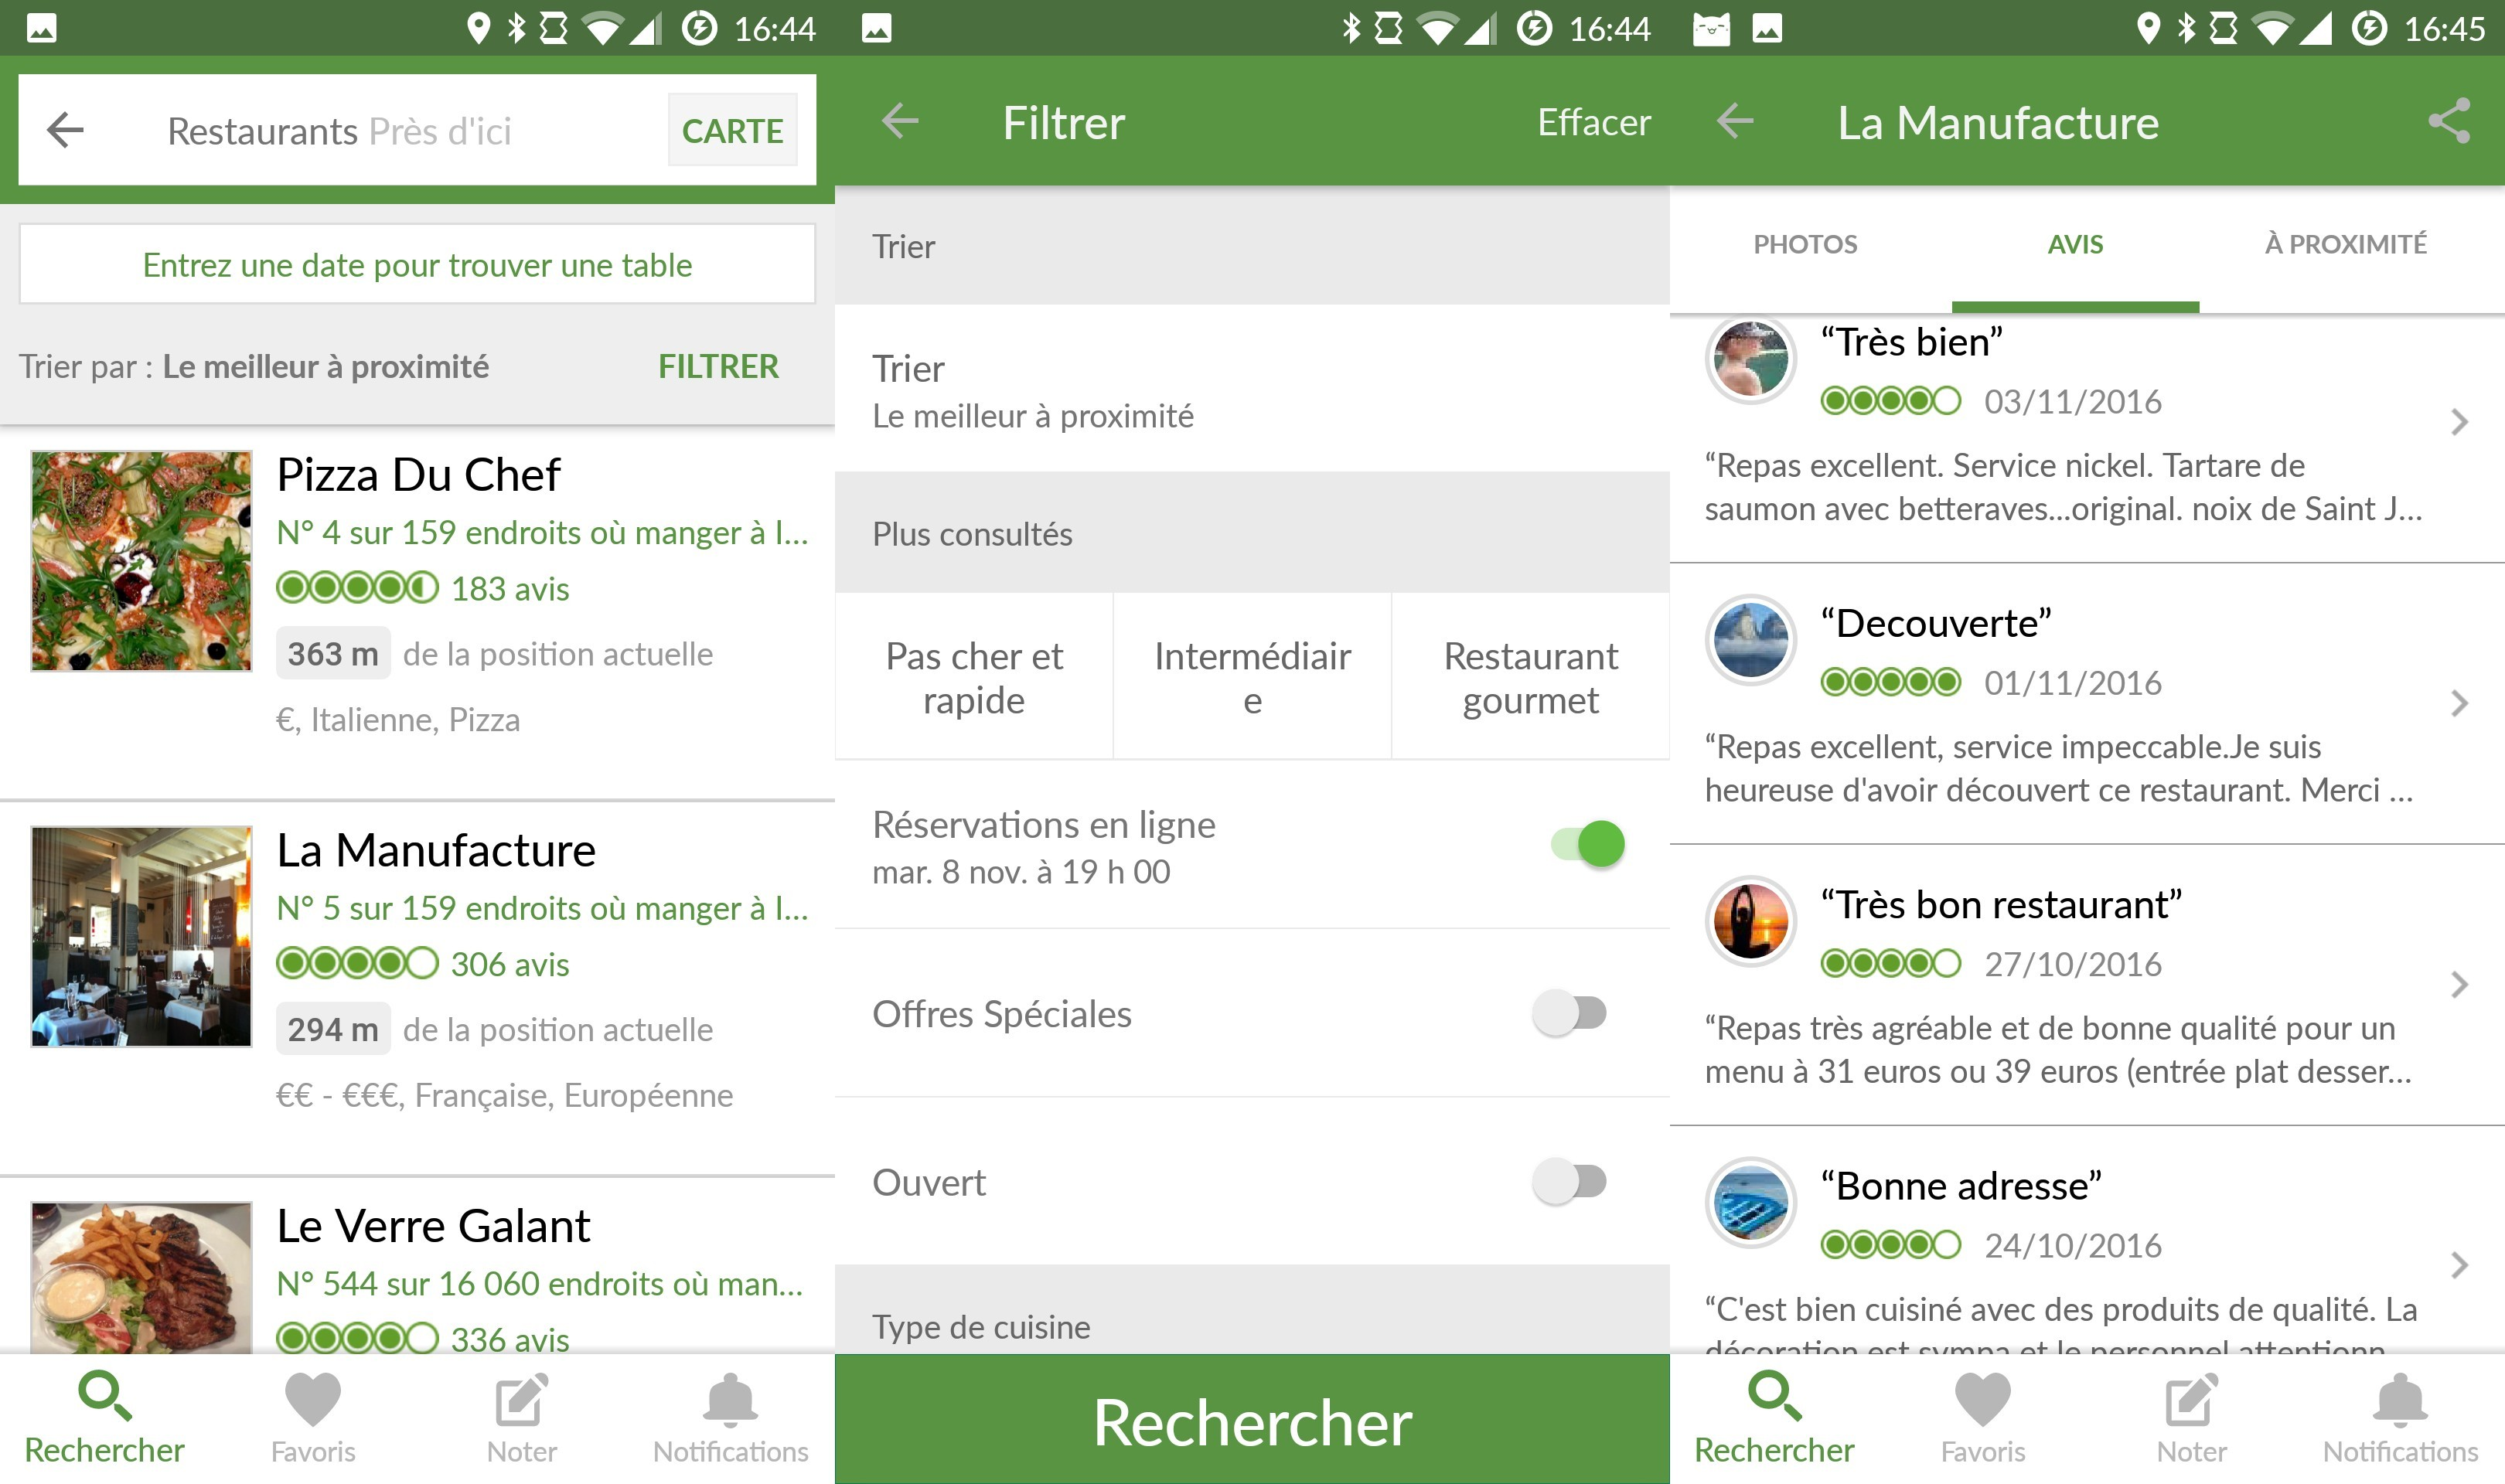
\includegraphics[width=4in]{images/Chapitre1/trip_advisor.jpeg}
		\label{fig:tripadvisor}
		\caption{Interface de TripAdvisor lors de la recherche des restaurants et les avis}
	 \end{figure}
\newpage
\subsubsection{Google Maps}
\begin{wrapfigure}[8]{r}{2cm}
	\vspace{-15pt}
	
\includegraphics[width=2cm]{images/Chapitre1/googlemaps.png}
	\vspace{-20pt}
	\caption{{\footnotesize Logo de Google Maps}}
 \end{wrapfigure}
Google maps est un service de cartographie développé par l'entreprise Google et lancé en 2005. Ce service offre différents types de vues et permet aussi d'afficher les différents points d'intérêts dans le monde comme les hôtels, les lieux d'attractions, etc. Ce qui nous intéresse dans notre domaine de recherche est la géolocalisation des restaurants, une fonctionnalité qu'offre ce service.

En accédant au site web ou l'application mobile, l'utilisateur aura accès à un large choix de restaurants proposés grâce à un système de suggestions, aussi développé par Google. L'utilisateur pourra donc accéder aux informations des restaurants ainsi que des photos et des avis généralement postés par la communauté des utilisateurs de Google Maps.
\subparagraph*{}
Google Maps présente de nombreux avantages, nous en citerons :\bigskip
 
	\tab- L'utilisation de ce service est gratuite.\medskip

	\tab- La plupart des restaurants sont affichés dans la carte.\medskip

	\tab- Les images des restaurants sont parfois affichées.\medskip
	
	\tab- Les utilisateurs peuvent donner des avis et des notes.\medskip

	\tab- Des itineraires precis sont proposés.\bigskip

	
Néanmoins ce service présente aussi des inconvénients:\bigskip

	\tab- Les menus detaillés ne sont pas affichés dans l'interface.\medskip

	\tab- On ne peut pas filtrer les types de restaurants.\medskip


	\begin{figure}[!ht]

		\centering
		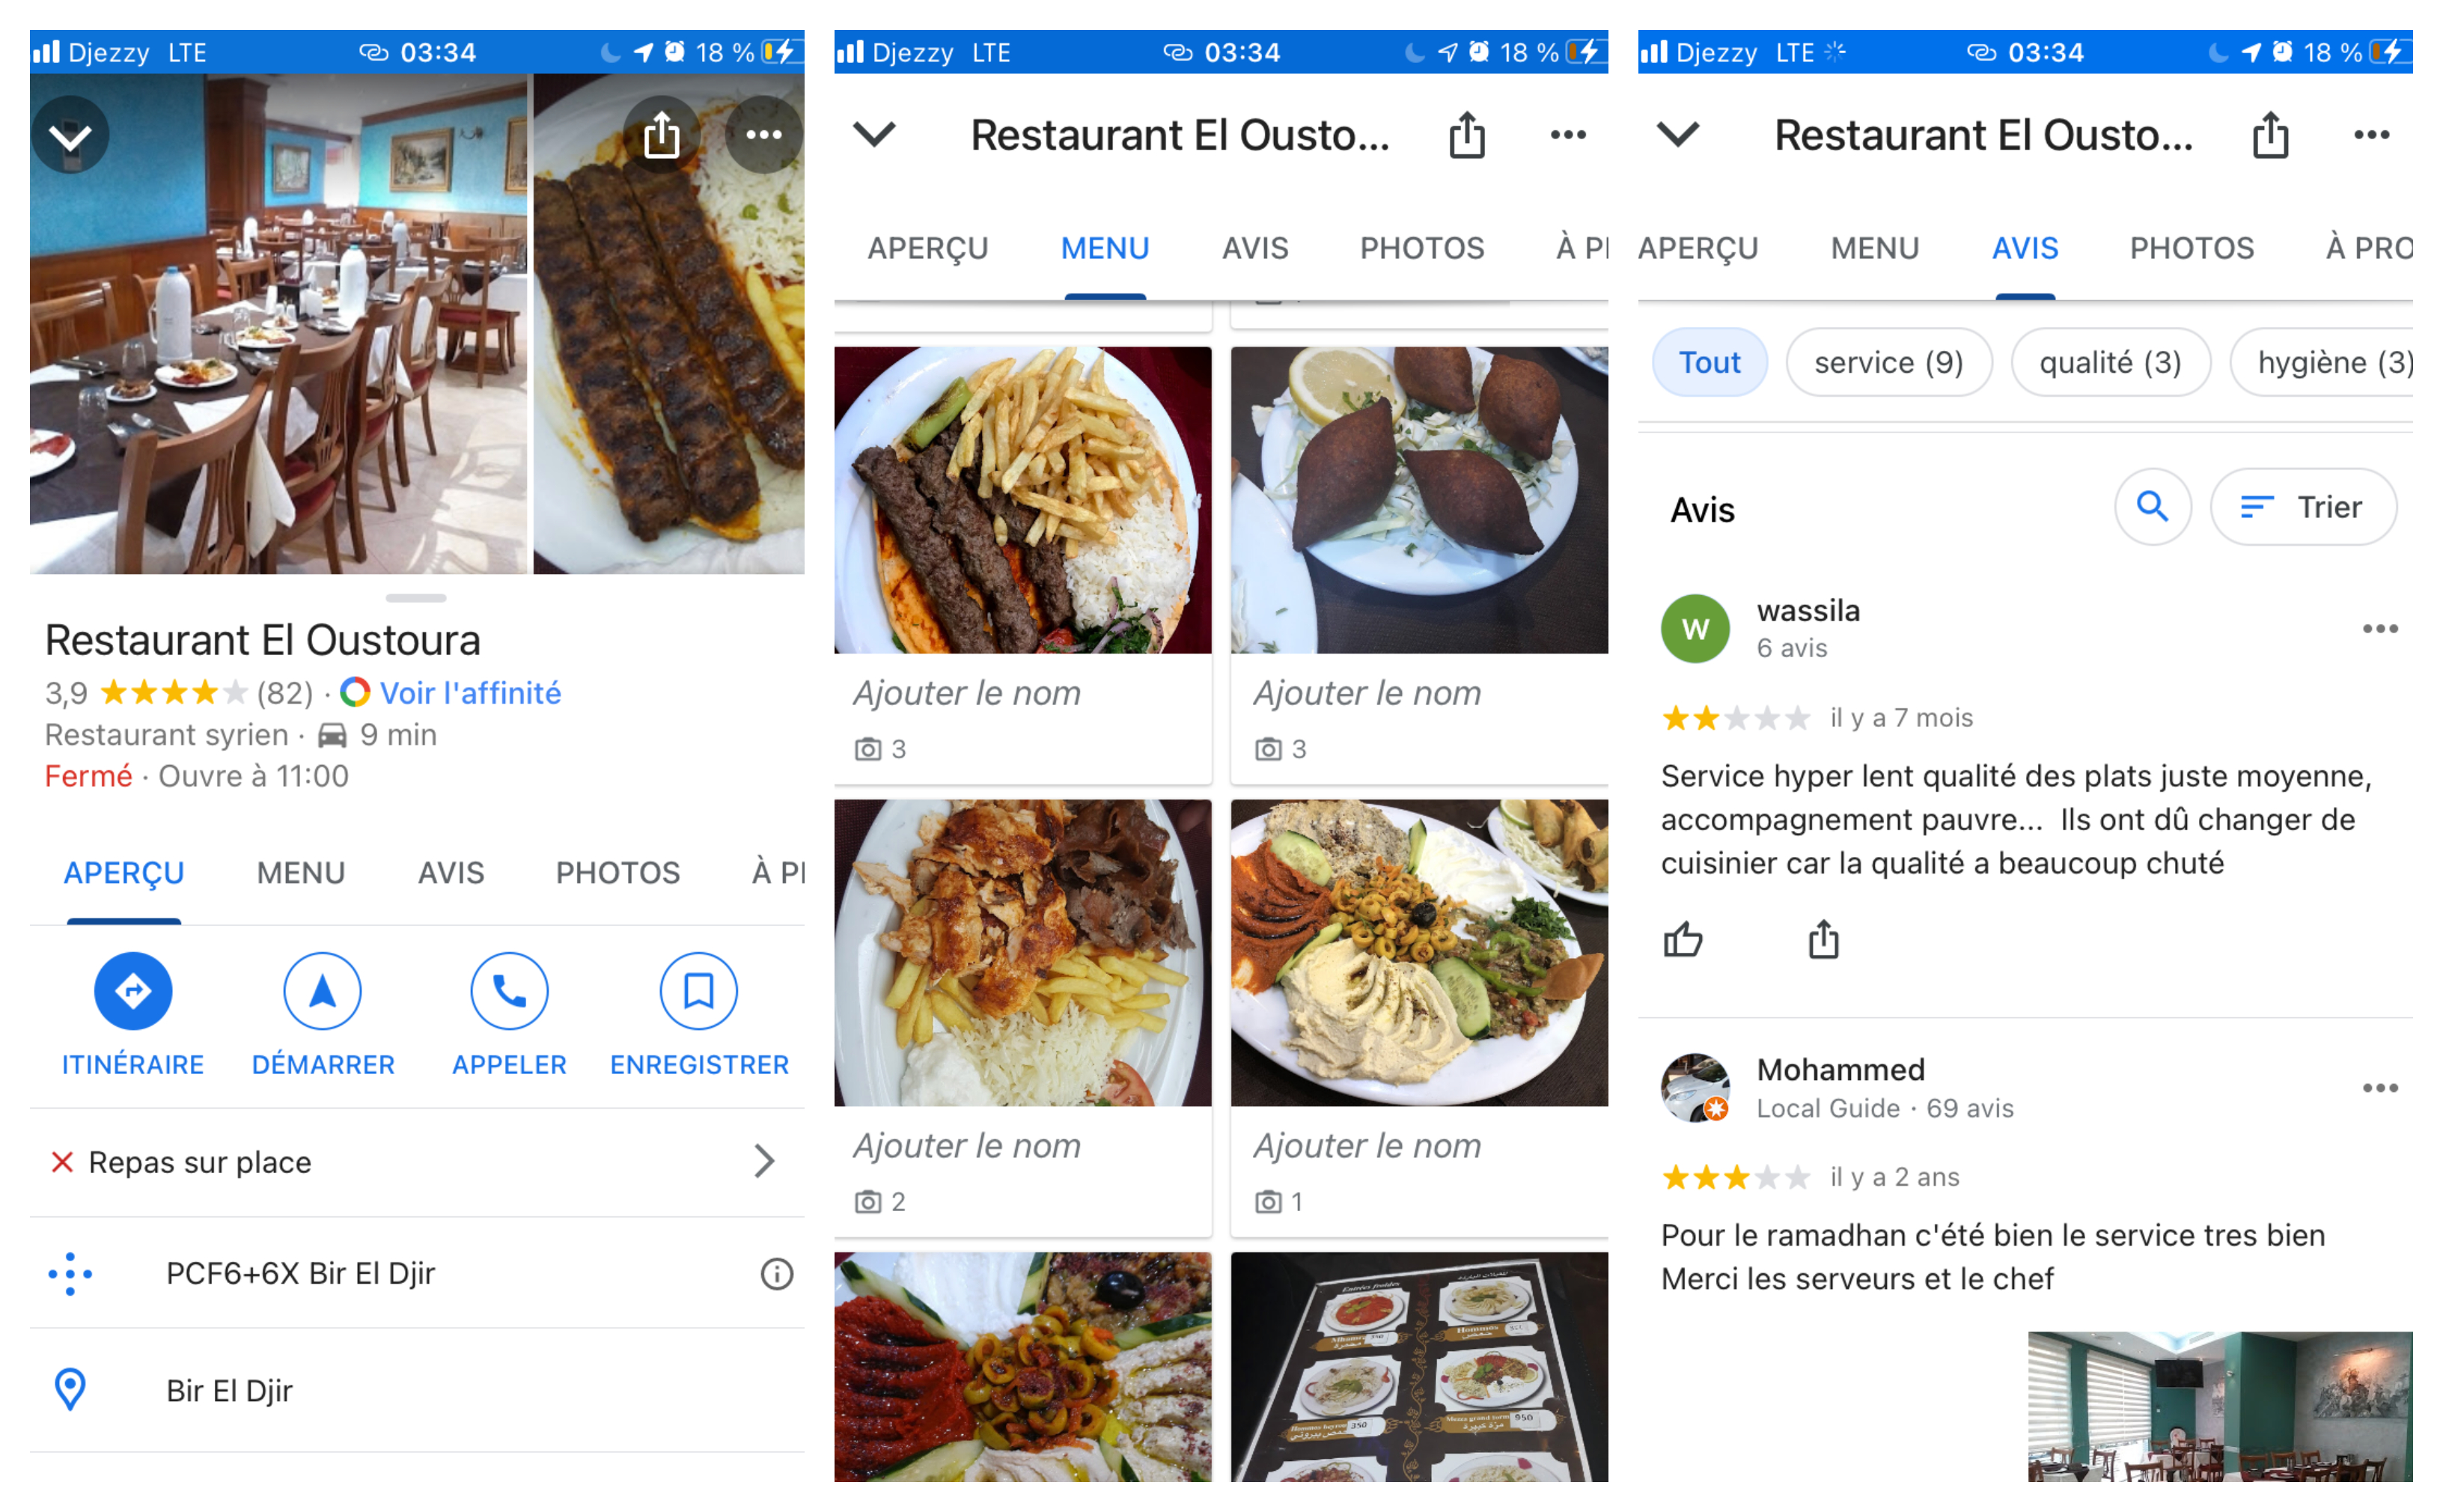
\includegraphics[width=4.5in]{images/Chapitre1/page_resto.jpg}
		\label{fig:pageresto}
		\caption{Exemple de différents ecrans lors d'une recherche d'un restaurant }
	 \end{figure}
	 
\newpage

\subsubsection{LaFourchette}
TheFork de son ancien nom "LaFourchette" est une plate-forme française de réservation de restaurants en ligne, accessible par un site web et par une application mobile disponible sur Android et iOS. Elle est présente dans plus de vingt pays en Europe et en Amérique latine.~\cite{TheFork2020}
\subparagraph*{}
\begin{wrapfigure}[8]{r}{3cm}
    \vspace{-15pt}
    
\includegraphics[width=3cm]{images/Chapitre1/lafourchette.jpg}
    \vspace{-20pt}
    \caption{{\footnotesize Logo de LaFourchette}}
\end{wrapfigure}

\subparagraph*{}
TheFork a ces avantages et ces inconvénients, parmi ces avantages on a :\bigskip

	\tab- La base de données regroupe plus de 80000 restaurants a travers le monde.~\cite{RestaurantsSiteReservation} \medskip

	\tab- L'application est multiplate-forme et disponible en version web et mobile. \medskip

	\tab- L'interface utilisateur est simple qui permet d'utiliser le service de manière efficace. \medskip

	\tab- La présence de la fonction d'exploration des restaurants via une carte.\bigskip

Quant aux Inconvénients nous citeront :\bigskip

	\tab- Le service n'est pas totalement gratuit.\medskip

	\tab- Cette application est dédiée qu'aux réservations de restaurans et ne donne pas des informations détaillées sur les menus.\medskip

	\tab- L'application ne prends pas encore en charge les restaurans algeriens. \medskip

   



\subsection{Les diagrammes UML}
Le langage UML est un langage de modélisation visuelle commun,
et riche sémantiquement et syntaxiquement. Il est destiné à 
l'architecture, la conception et la mise en œuvre de systèmes logiciels complexes par leur structure aussi bien que leur comportement.
Il ressemble aux plans utilisés dans d'autres domaines et se 
compose de différents types de diagrammes. Dans l'ensemble, 
les diagrammes UML décrivent la limite, la structure et le 
comportement du système et des objets qui s'y trouvent.

L'UML n'est pas un langage de programmation, mais il existe des outils qui peuvent être utilisés pour générer du code en plusieurs langages à partir de diagrammes UML. L'UML a une relation directe avec l'analyse et la conception orientées objet.\\
Pour bien expliquer le fonctionnement de notre application et modéliser les diagrammes. On a utilisé l'outil Visual Paradigm Online qui est facile à manipuler afin de réaliser ces diagrammmes.
\newpage
\subsubsection{Diagrammes de séquence}
Enchainement des actions pour le lancement de l'application
\begin{figure}[!ht]

    \centering
    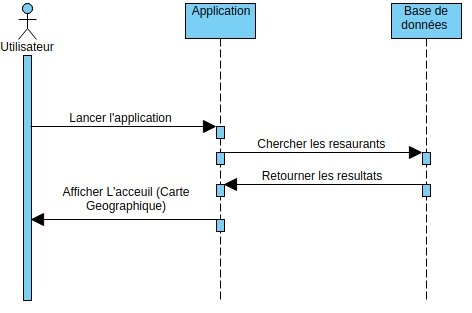
\includegraphics[width=5in]{images/Chapitre3/enchainement_lancement_application.jpg}
    \label{fig:umllancement}
    \caption{Enchainement des actions pour le lancement de l'application}
\end{figure}

\begin{figure}[!ht]

    \centering
    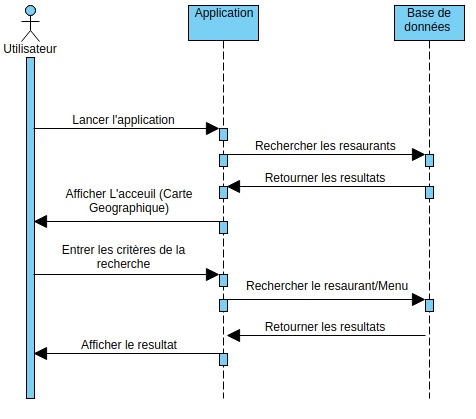
\includegraphics[width=4in]{images/Chapitre3/enchainement_recherche_resto_menu.jpg}
    \label{fig:label1}
    \caption{Enchainement des actions pour la recherche des restaurants}
\end{figure}

\begin{figure}[!ht]

    \centering
    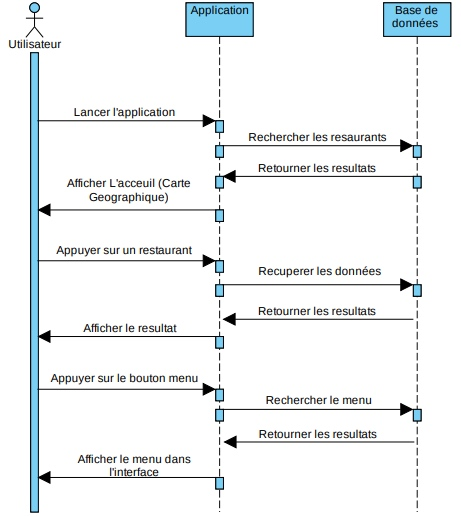
\includegraphics[width=3in]{images/Chapitre3/enchainement_affichage_resto_menu.jpg}
    \label{fig:label2}
    \caption{Enchainement des actions pour l'affichage de la page restaurant et son menu}
\end{figure}

\newpage
\subsubsection{Diagramme d'action}
\begin{figure}[!ht]

    \centering
    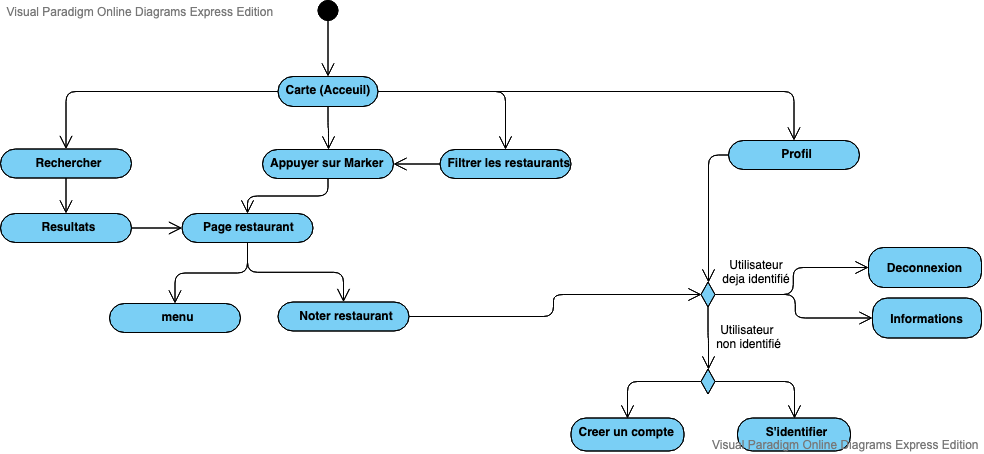
\includegraphics[width=6in]{images/Chapitre3/Diagramme_action.png}
    \label{fig:label3}
    \caption{Diagramme d'actions}
\end{figure}


\newpage
\subsection{Maquette fonctionelle (Wireframe)}
\subsubsection{Définition} La maquette fonctionelle ou Wireframe est
un schéma utilisé lors de la conception des interfaces des applications
pour définir les emplacements des  zones de texte, des images, des vidéos, des liens,
ainsi que des différents éléments graphiques.
\subsubsection{Outil utilisé}
Balsamiq Wireframes est une application de création d'interface 
utilisateur graphique ,elle permet au concepteur d'organiser des 
widgets prédéfinis à l' aide d'un éditeur WYSIWYG par glisser-
déposer .L'application est proposée dans une version de bureau 
ainsi qu'un plug-in pour Google Drive ~\cite{Balsamiq2020}.
\begin{figure}[!h]

    \centering
    
\includegraphics[width=4cm]{images/Chapitre3/balmockups.png}
    \label{fig:logobalsamiq}
    \caption{Logo de Balsamiq}
\end{figure}
\begin{figure}[!h]

    \centering
    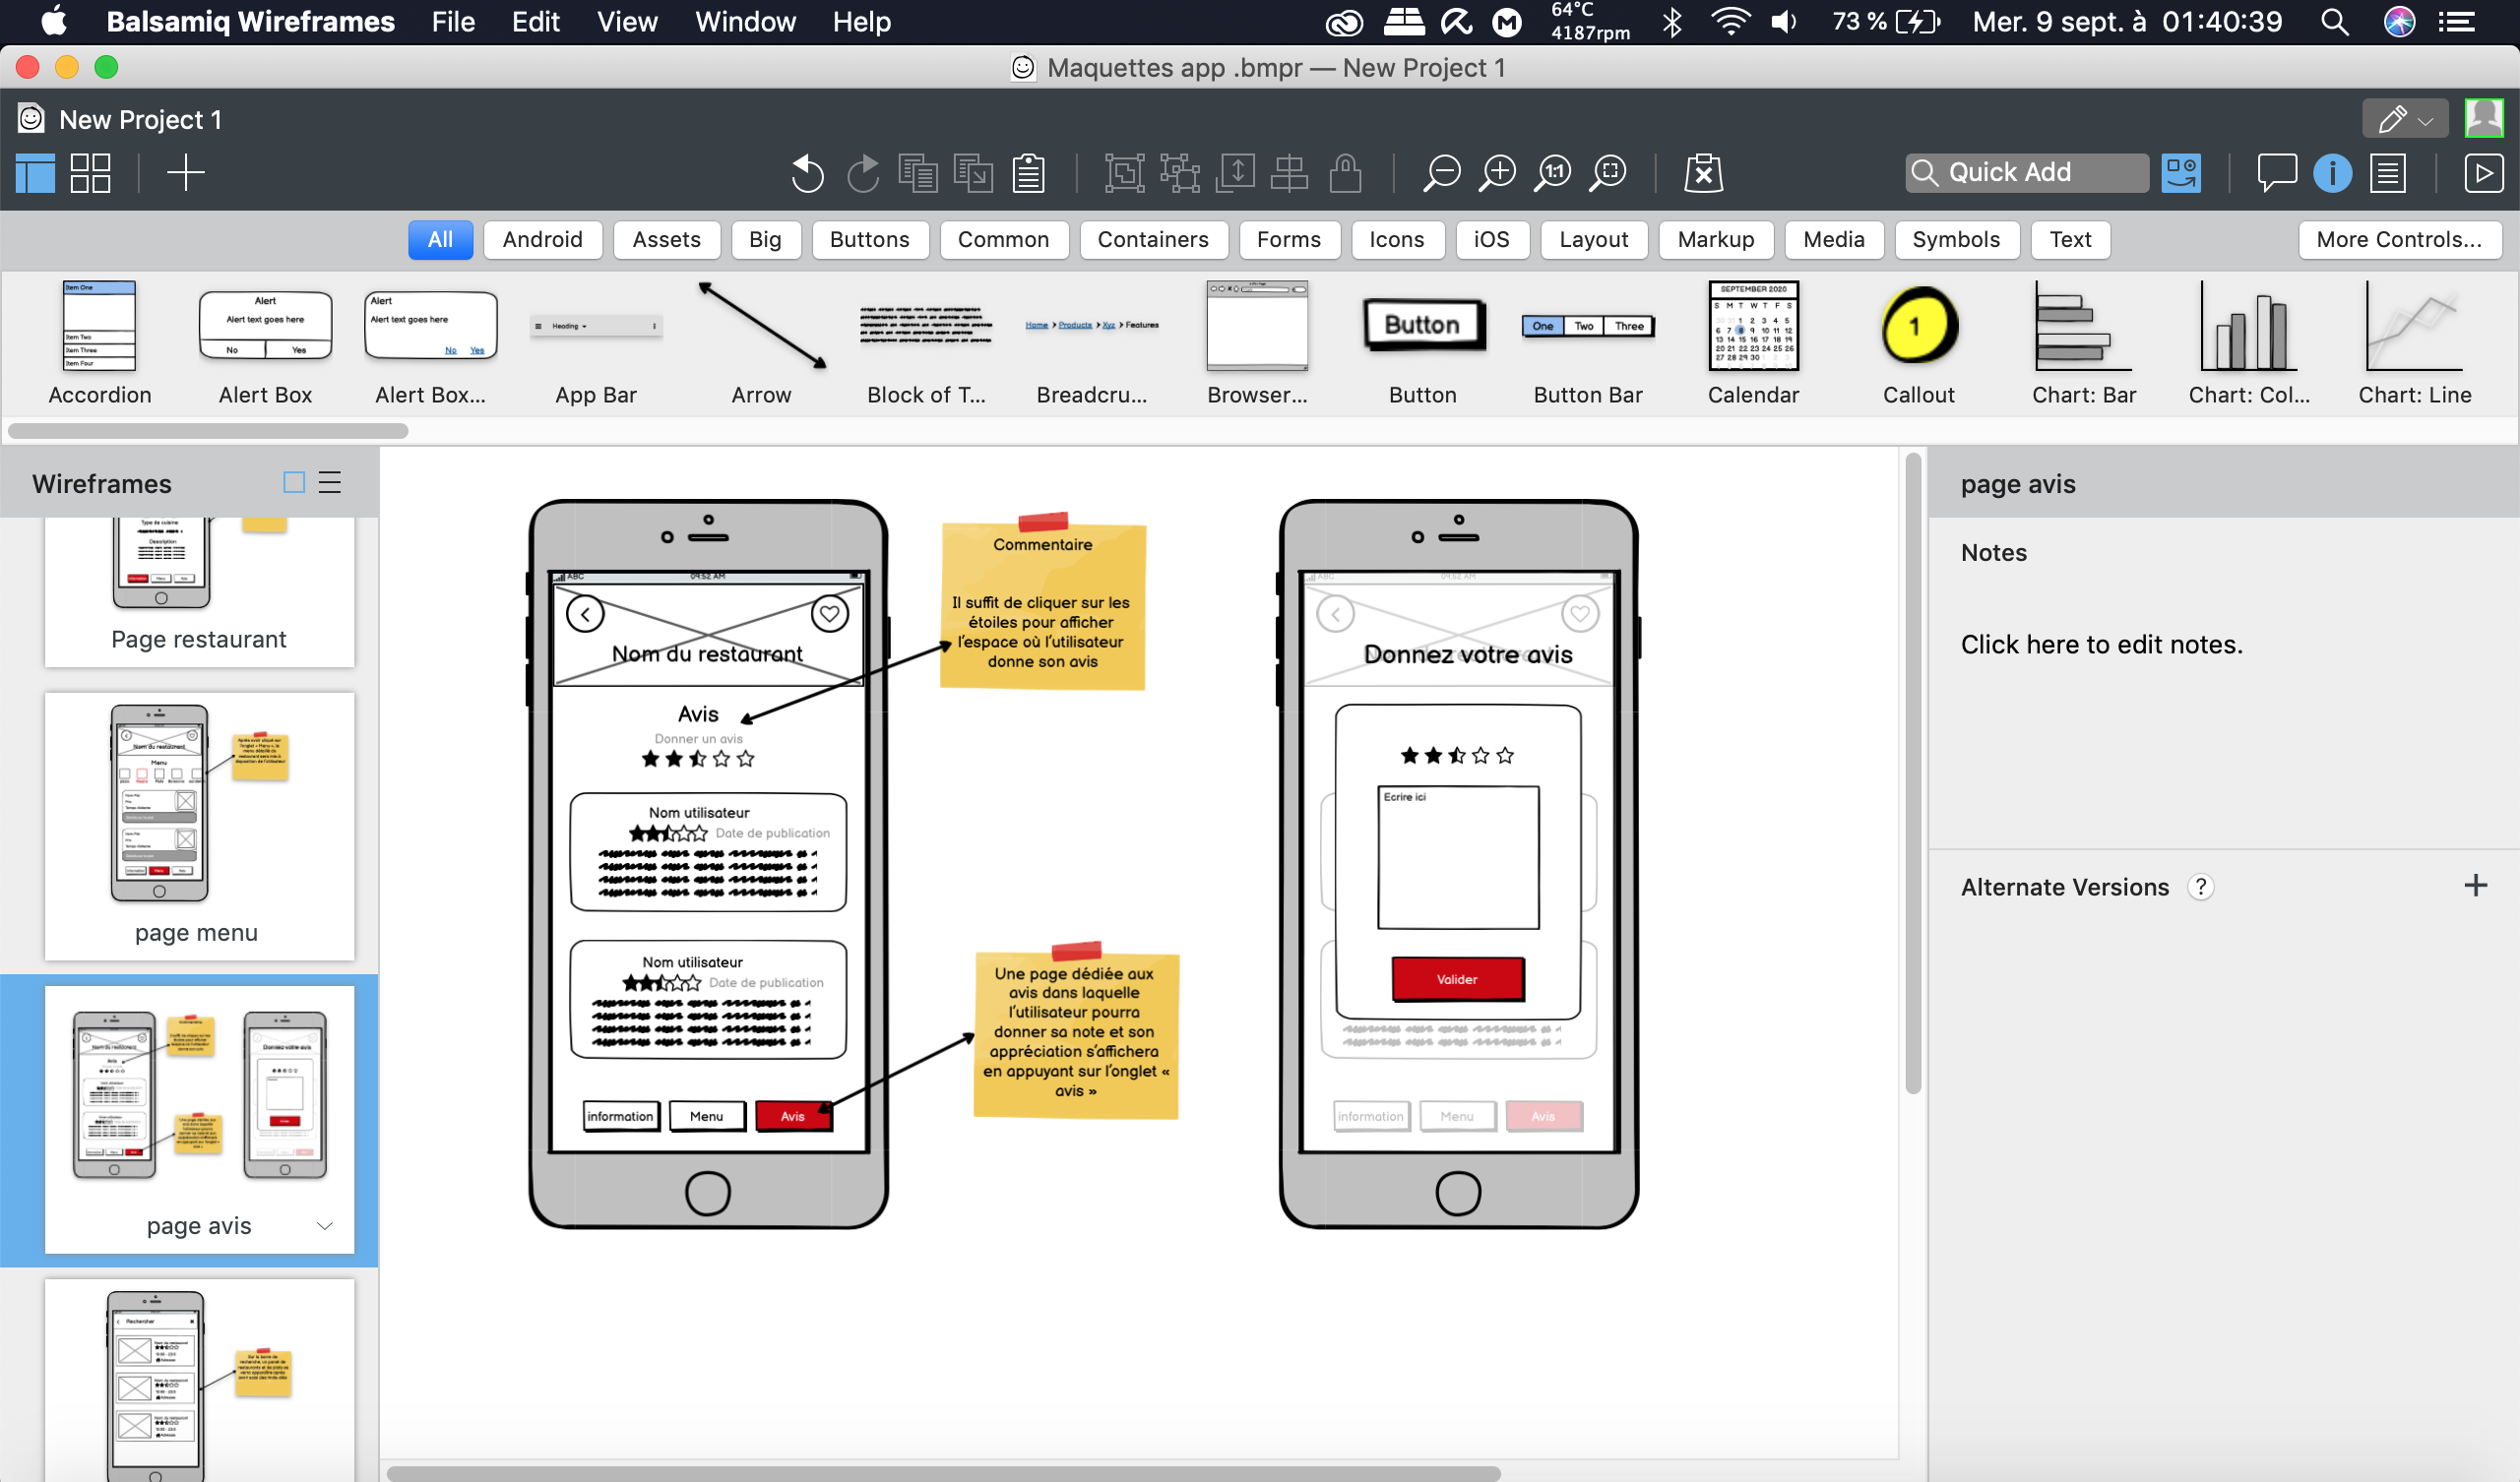
\includegraphics[width=6in]{images/Chapitre3/interface_balsamiq.png}
    \label{fig:interfacebalsamiq}
    \caption{Interface du logiciel Balsamiq}
\end{figure}
\newpage
\subsubsection{Les différents ecrans}
\begin{figure}[!h]
    \centering
    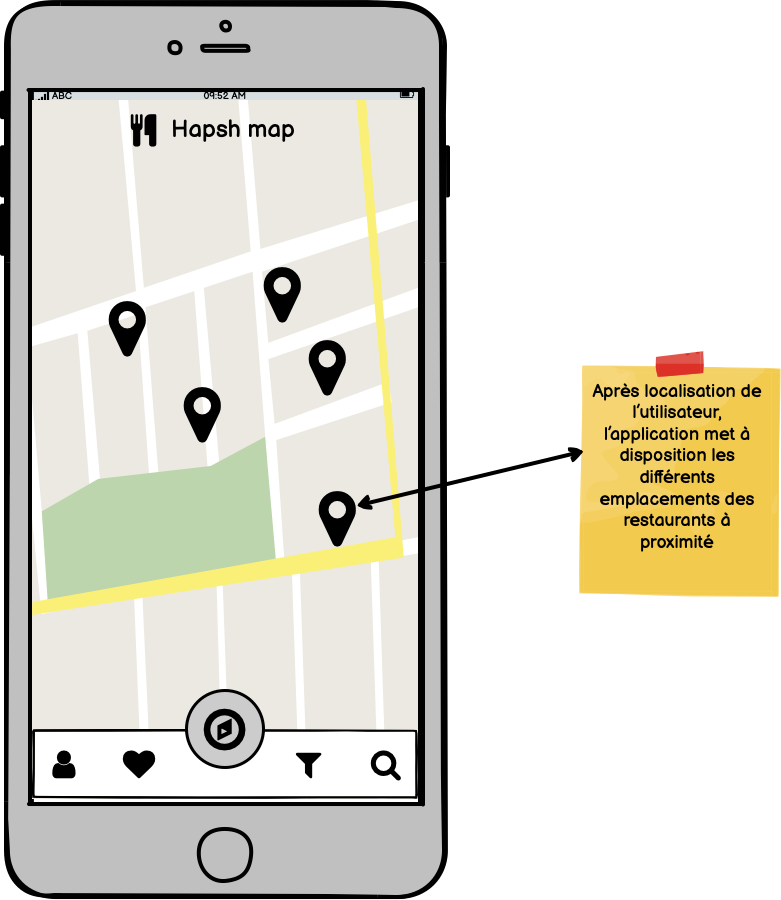
\includegraphics[width=8cm]{images/Chapitre3/maquettes_balsamiq/Acceuil.png}
    \label{fig:acceuil}
    \caption{Ecran principal}
\end{figure} 
\begin{figure}[!h]
    \centering
    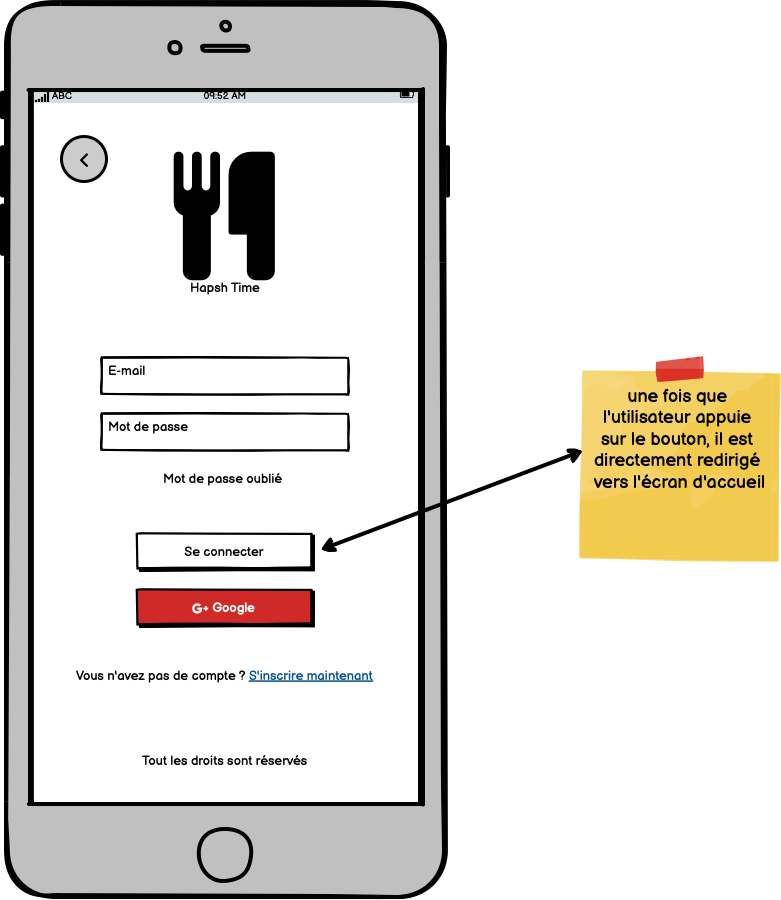
\includegraphics[width=8cm]{images/Chapitre3/maquettes_balsamiq/Connection.png}
    \label{fig:connexion}
    \caption{Ecran de connexion}
\end{figure} 
\newpage
\begin{figure}[!h]
    \centering
    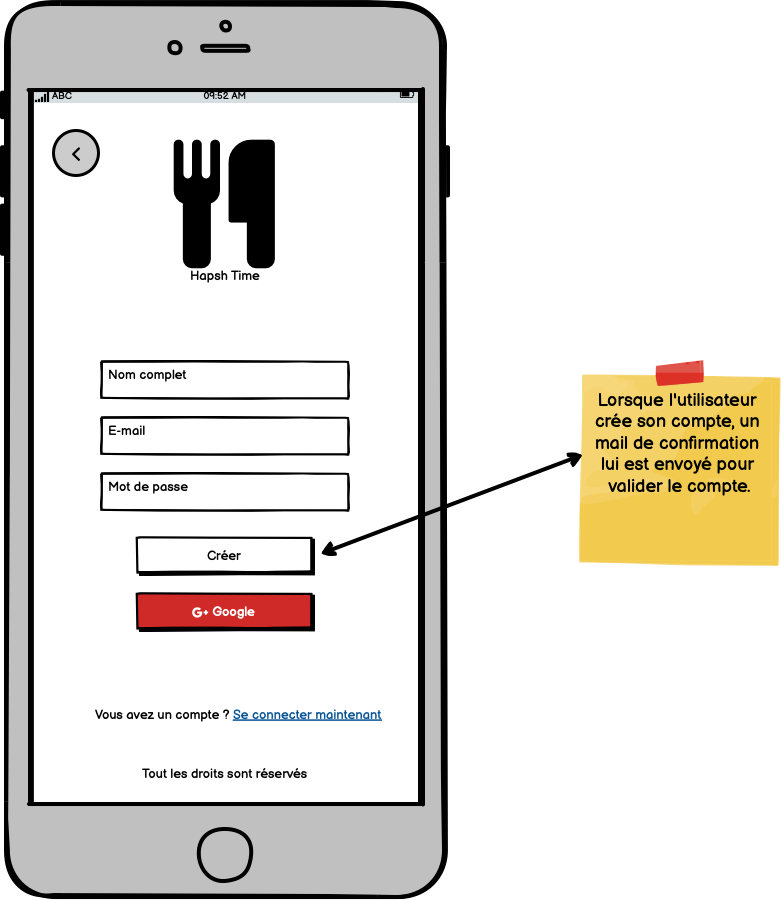
\includegraphics[width=8cm]{images/Chapitre3/maquettes_balsamiq/Creer.png}
    \label{fig:creation}
    \caption{Ecran de creation du compte}
\end{figure} 
\begin{figure}[!h]
    \centering
    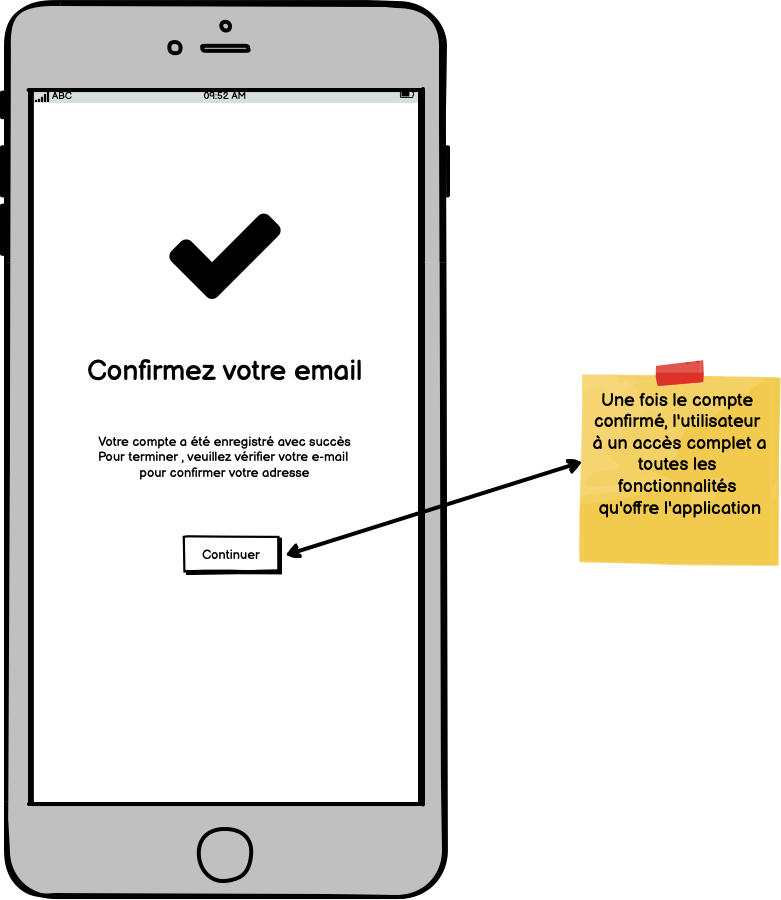
\includegraphics[width=8cm]{images/Chapitre3/maquettes_balsamiq/Confirmation.png}
    \label{fig:confirmation}
    \caption{Ecran de confirmation du compte}
\end{figure} 
\newpage
\begin{figure}[!h]
    \centering
    \includegraphics[width=8cm]{images/Chapitre3/maquettes_balsamiq/mot_de_passe_oublié.png}
    \label{fig:mdpoublié}
    \caption{Ecran de réinitialisation du mot de passe}
\end{figure} 
\begin{figure}[!h]
    \centering
    \includegraphics[width=8cm]{images/Chapitre3/maquettes_balsamiq/Restaurant_card.png}
    \label{fig:restocard}
    \caption{Ecran d'affichage de la fenêtre du restaurant}
\end{figure} 
\newpage
\begin{figure}[!h]
    \centering
    \includegraphics[width=8cm]{images/Chapitre3/maquettes_balsamiq/Page_restaurant.png}
    \label{fig:pageresto}
    \caption{Page de détails du restaurant}
\end{figure} 
\begin{figure}[!h]
    \centering
    \includegraphics[width=8cm]{images/Chapitre3/maquettes_balsamiq/page_menu .png}
    \label{fig:pagemenu}
    \caption{Page de détails du menu}
\end{figure} 
\newpage
\begin{figure}[!h]
    \centering
    \includegraphics[width=14cm]{images/Chapitre3/maquettes_balsamiq/page_avis.png}
    \label{fig:pageavis}
    \caption{Page d'avis}
\end{figure} 
\begin{figure}[!h]
    \centering
    \includegraphics[width=8cm]{images/Chapitre3/maquettes_balsamiq/Page_de_recherche.png}
    \label{fig:pagerecherche}
    \caption{Page de recherche}
\end{figure} 
\newpage
\begin{figure}[!h]
    \centering
    \includegraphics[width=10cm]{images/Chapitre3/maquettes_balsamiq/Profil.png}
    \label{fig:profil}
    \caption{Page du profil et parametres}
\end{figure} 
\newpage
\begin{figure}[!h]
    \centering
    \includegraphics[width=8cm]{images/Chapitre3/maquettes_balsamiq/Filtre.png}
    \label{fig:filtre}
    \caption{Page du filtre}
\end{figure} 
\begin{figure}[!h]
    \centering
    \includegraphics[width=8cm]{images/Chapitre3/maquettes_balsamiq/favorite_restaurants.png}
    \label{fig:favoris}
    \caption{Page des restaurants favoris}
\end{figure} 
\newpage
\subsection{Prototypage et interface utilisateur}
La phase de Prototypage et de la création de l'interface utilisateur est une étape très importante dans le développement des applications mobiles. pour ce projet on a utilisé les règles de design appelées le material design de Google qui est un design très présent dans les applications mobiles en ce temps.
\subsubsection{Material design}
Le Material Design est un ensemble de règles de design proposées par Google et qui s'appliquent a l'interface graphique 
des logiciels et applications . Il est utilisé notamment a partir de la verison 5.0 (Lolipop) du systéme d'exploitation 
Android.

Google a présenté le Material Design pour la première fois lors de la conférence Google I/O, le 25 juin 2014. Ces régles 
de design mettent l'accent sur une utilisation accrue des mises en page basées sur une grille , des animations et des
transitions, des effets de profondeur tels l'éclairage et les ombres. Selon Google ce nouveau language de design est basé 
sur le papier et l'encre.

Le designer Matías Duarte explique que « contrairement au vrai papier, notre matériau numérique peut s'étirer et se 
modifier de manière intelligente. Le matériau contextuel a une surface physique et des bords. Les superpositions et 
les ombres donnent des informations sur ce que vous pouvez toucher ».~\cite{MaterialDesign2020}
\begin{figure}[!h]

    \centering
    \includegraphics[width=5in]{images/Chapitre3/material design.png}
    \label{fig:label5}
    \caption{Exemple de composantes du Material Design}
\end{figure}
\subsubsection{Outil utilisé (Adobe XD)}
Adobe XD est unoutil de conception de l' expérience utilisateur pour les applications Web et des applications mobiles , développé et édité par Adobe Inc . Il est disponible pour macOS et Windows , bien qu'il existe des versions pour iOS et Android pour aider à prévisualiser le résultat du travail directement sur les appareils mobiles. XD prend en charge le wireframing de site Web et la création de prototypes de clic ~\cite{AdobeXD2020}.
\begin{figure}[!h]

    \centering
    \includegraphics[width=3cm]{images/Chapitre3/AdobeXD.png}
    \label{fig:label6}
    \caption{Logo de Adobe XD}
\end{figure}
\begin{figure}[!h]

    \centering
    \includegraphics[width=6.5in]{images/Chapitre3/interface_adobe_xd.png}
    \label{fig:label6}
    \caption{interface du logiciel Adobe XD}
\end{figure}

\newpage
\subsubsection{Les Maquettes UI/UX}
\begin{figure}[!h]

    \centering
    \includegraphics[width=6.5in]{images/Chapitre3/maquettes_balsamiq/p1.jpg}
    \label{fig:ux1}
   
\end{figure}
\newpage
\begin{figure}[!h]

    \centering
    \includegraphics[width=6.5in]{images/Chapitre3/maquettes_balsamiq/p2.jpg}
    \label{fig:ux2}
   
\end{figure}
\newpage
\begin{figure}[!h]

    \centering
    \includegraphics[width=6.5in]{images/Chapitre3/maquettes_balsamiq/p3.jpg}
    \caption{Interfaces utilisateur de l'application}

    \label{fig:ux3}
   
\end{figure}
\newpage
\section{Implementation}
\subsection{Outils Materiels}
Le développement de cette application a ete effectue sur deux machines en parallèle avec les configurations suivantes :
\\
\textbf{Machine principale}

\begin{itemize}
    \item Marque : Lenovo Thinkpad
    \item Syeteme d'exploitation : Windows 10
    \item Microprocesseur : Intel Core i5
    \item Mémoire vice : 8 Go
    \item Disque dur : 256 GO SSD
          
\end{itemize}
\textbf{Machine secondaire}
\begin{itemize}
    \item Marque : Dell .
    \item Syeteme d'exploitation : Ubuntu 19.10.
    \item Microprocesseur : Intel Core i5.
    \item Mémoire vice : 8 Go.
    \item Disque dur : 1 To HDD+ 480 SSD.
\end{itemize}
Les tests de cette application  ont ete effectué sous un Emulateur Android PIXEL 3 et un Smartphone Galaxy j3 Pro sous Android 9
\newpage
\subsection{Outils Logiciels}
\subsubsection{Visual Studio Code}
Visual studio code est un éditeur de code cross-platform, open source et gratuit, supportant une dizaine de langages développés par Microsoft pour Windows, Linux et macos. Il facilite grandement le codage grâce à ses capacités à comprendre le code et aussi la navigation facile entre les différentes parties de code.
\begin{figure}[!h]
    \centering
    \includegraphics[width=4cm]{images/Chapitre3/vscode.png}
    \label{fig:label7}
    \caption{Logo de Visual studio code}
\end{figure}
\begin{figure}[!h]

    \centering
    \includegraphics[width=6in]{images/Chapitre3/interface_vs_code.png}
    \label{fig:interfacevscode}
    \caption{Interface du logiciel Visual Studio Code}
\end{figure}
\newpage
\subsection{Developpement}
\subsubsection{Base de données}
Pour la base de données nous avons choisi d'utiliser le service de base de données fourni par
firebase avant d'aller plus dans le détail définissons firebase.

\textbf{Firebase}
Firebase est un ensemble de services d'hébergement pour n'importe quel type 
d'application (Android, iOS, Javascript, Node.js, Java, Unity, PHP, C++ ...).
Il propose d'héberger en NoSQL et en temps réel des bases de données, du contenu,
de l'authentification sociale (Google, Facebook, Twitter et Github), et des 
notifications, ou encore des services, tel que par exemple un serveur de 
communication temps réel.~\cite{Firebase2020}

\begin{figure}[!h]
    \centering
    \includegraphics[width=8cm]{images/Chapitre3/firebase.png}
    \label{fig:label8}
    \caption{Logo de Firebase}
\end{figure}  
\begin{figure}[!h]

    \centering
    \includegraphics[width=7in]{images/Chapitre3/firebase_console.png}
    \label{fig:firebasepricing}
    \caption{Interface de la console de Firebase }
\end{figure}

\newpage
\subsubsection{Les packages utilisés: }         
\textbf{Google maps flutter:}\\
Avec le plugin Google Maps Flutter, on peut ajouter des cartes basées sur les données de Google Maps ànotre application. Le plugin gère automatiquement l'accès aux serveurs Google Maps, l'affichage de la carte et la réponse aux gestes de l'utilisateur tels que les clics et les traînées. On peut également ajouter des marqueurs à notre carte. Ces objets fournissent des informations supplémentaires sur les emplacements de la carte et permettent à l'utilisateur d'interagir avec la carte.\bigskip

\textbf{Cloud Firestore:}\\
Ce package permet d'intégrer les services de base de données NoSQL de Firebase pour l'utilisation en temps réel. Les données sont stockées dans l'arborescence JSON sous la forme des collections, où chaque collection un nombre infini de documents, ces derniers contiennent les données de la base de données.\bigskip

\textbf{Geolocator: }\\
Geolocator est un plugiciel de géolocalisation dédié à Flutter, ce dernier offre un accès facile au service de localisations spécifiques à la plateforme.\bigskip

Geolocator permet de: 
\begin{itemize}
    \item Obtenir le dernier emplacement de l'utilisateur.
    \item Obtenir l'emplacement actuel de l'appareil.
    \item Vérifier si les services de localisation sont activés sur l'appareil.
    \item Calculer la distance (en mètres) entre deux points géographique.
\end{itemize}
\bigskip

\textbf{Firebase auth:}\\
Firebase auth est un plugin Flutter pour utiliser l'API d'authentification Firebase. Cet APi permet de gérer les authentifications des utilisateurs en offrant differentes options d'inscription et de connexion a leurs comptes.\bigskip

\textbf{Goole sign in:}\\
Google sign in est un plugin Flutter qui offre un système d'authentification sécurisé pour se connecter avec un compte Google sur Android et iOS.\bigskip
 \chapter{Conslusion et perspectives}
Dans ce rapport, nous avons exposé les étapes
de conception et de développement de notre 
application qui consiste à créer une application
mobile pour la geolocalisation des restaurants 
dans la ville d'oran .
\\
\\
Notre travail s'est déroulé sur trois étapes. nous avons commencé par une étude des applications mobiles et différents systèmes d'exploitation
\\
\\
Dans la deuxiéme phase, nous avons abordé les différentes technologies utilisés, on a commencé par Flutter, ensuite Firebase et a la fin on a parlé des API de Google.
\\
\\
Dans la troisième étape , nous avant spécifié l'objectif du projet ainsi qu'une étude de l'existant. Ensuite on est passé a l'étape conception 
en utilisant des diagrammes UML et actions ainsi que les maquettes et interfaces utilisateur ,enfin l'implementation de notre 
code.
\\
\\
Ce projet se situe en effet , dans le cadre du projet de
fin d'etude de license en informatique. Ce projet était une 
veritable expérience de travail en collaboration, qui nous a permis
de bien gérer la répartition des taches et de renforcer l'esprit 
de partage de connaissances ainsi que la synchronisation de 
notre travail.
\\
\\
Cependant, nous pouvons encore améliorer cette application 
en creant une application web  et aussi integrer un systeme 
d'intelligence artificielle qui permet de proposer du contenu 
adapté a l'utilisateur .

\bibliography{biblio}
\bibliographystyle{plain}

\input{Parts/resume.tex}


\end{document}